\documentclass[preprint,12pt]{elsarticle}
\biboptions{numbers,sort&compress}
\usepackage[english]{babel}
\usepackage{lmodern}
\usepackage{graphicx}
\usepackage{booktabs}
\usepackage{adjustbox}
\usepackage[htt]{hyphenat}
\usepackage{amsmath,amssymb}
\usepackage{enumitem}
\usepackage{algorithm}
\usepackage{algpseudocode}
\usepackage{siunitx}
\usepackage{xurl}
\usepackage[hidelinks]{hyperref}
\graphicspath{{../}}
% Auto-generated by scripts/make_numbers_tex.py -- do not edit by hand.
\newcommand{\BasisStorage}{158{,}400}
\newcommand{\CondConfTen}{274{,}505}
\newcommand{\CondConfThirty}{1{,}071}
\newcommand{\CondDgTen}{3{,}757}
\newcommand{\CondDgThirty}{1{,}071}
\newcommand{\CondRandTen}{38{,}981}
\newcommand{\CondRandThirty}{1{,}071}
\newcommand{\CostBlockDg}{3.2}
\newcommand{\CostLoneWell}{32}
\newcommand{\CostLsWell}{0.8}
\newcommand{\CostPodSvd}{1.18}
\newcommand{\CostQr}{2.1}
\newcommand{\CostQrDg}{1.0}
\newcommand{\CostSynth}{4.8}
\newcommand{\CostTucker}{8.9}
\newcommand{\CrossSdEnd}{1.17}
\newcommand{\CrossSdMax}{1.68}
\newcommand{\DevCorrMax}{-0.17}
\newcommand{\DevCorrMin}{-0.39}
\newcommand{\DevSdMax}{1.06}
\newcommand{\DevSdMin}{0.32}
\newcommand{\DevShiftMax}{1.86}
\newcommand{\DevShiftMin}{0.18}
\newcommand{\EOnePOneFloorRatio}{20}
\newcommand{\EOnePOnePodOracle}{0.014}
\newcommand{\EOnePOnePriorP}{0.191}
\newcommand{\EOnePOneRoneFortyeight}{0.287}
\newcommand{\EOnePOneRoneFull}{0.014}
\newcommand{\EOnePOneRoneNinetysix}{0.015}
\newcommand{\EOnePOneRoneTwelve}{2.059}
\newcommand{\EOnePOneRoneTwentyfour}{1.187}
\newcommand{\EOnePOneTbmdOracle}{0.29}
\newcommand{\EOnePTwoFloorRatio}{6}
\newcommand{\EOnePTwoPodOracle}{0.056}
\newcommand{\EOnePTwoPriorP}{1.148}
\newcommand{\EOnePTwoRoneFortyeight}{0.354}
\newcommand{\EOnePTwoRoneFull}{0.056}
\newcommand{\EOnePTwoRoneNinetysix}{0.057}
\newcommand{\EOnePTwoRoneTwelve}{2.482}
\newcommand{\EOnePTwoRoneTwentyfour}{1.431}
\newcommand{\EOnePTwoTbmdOracle}{0.35}
\newcommand{\EZeroErrOne}{0.051}
\newcommand{\EZeroErrTen}{0.023}
\newcommand{\EZeroPsnrOne}{33.1}
\newcommand{\EZeroPsnrTen}{37.5}
\newcommand{\EZeroSsimOne}{0.998}
\newcommand{\EZeroSsimTen}{0.999}
\newcommand{\LoneConfTen}{0.314}
\newcommand{\LoneConfThirty}{0.19}
\newcommand{\LoneDgTen}{0.351}
\newcommand{\LoneDgThirty}{0.19}
\newcommand{\LoneRandTen}{0.307}
\newcommand{\LoneRandThirty}{0.19}
\newcommand{\NActive}{4{,}950}
\newcommand{\NInactive}{1{,}722}
\newcommand{\NRuns}{10}
\newcommand{\NT}{133}
\newcommand{\NTestPOne}{27}
\newcommand{\NTrainPOne}{106}
\newcommand{\NWells}{30}
\newcommand{\NoiseWellTenConfLoneSigOne}{0.55}
\newcommand{\NoiseWellTenConfLoneSigTwo}{1.07}
\newcommand{\NoiseWellTenConfLoneSigZero}{0.31}
\newcommand{\NoiseWellTenConfLsSigOne}{188.0}
\newcommand{\NoiseWellTenConfLsSigTwo}{458.2}
\newcommand{\NoiseWellTenConfLsSigZero}{2.5}
\newcommand{\NoiseWellTenIdwSigOne}{0.75}
\newcommand{\NoiseWellTenIdwSigTwo}{1.09}
\newcommand{\NoiseWellTenIdwSigZero}{0.58}
\newcommand{\NoiseWellTenPodeLoneSigOne}{0.60}
\newcommand{\NoiseWellTenPodeLoneSigTwo}{1.18}
\newcommand{\NoiseWellTenPodeLoneSigZero}{0.35}
\newcommand{\NoiseWellTenPodeLsSigOne}{5.68}
\newcommand{\NoiseWellTenPodeLsSigTwo}{14.01}
\newcommand{\NoiseWellTenPodeLsSigZero}{0.78}
\newcommand{\NoiseWellTenTbmdLoneSigOne}{0.77}
\newcommand{\NoiseWellTenTbmdLoneSigTwo}{1.25}
\newcommand{\NoiseWellTenTbmdLoneSigZero}{0.64}
\newcommand{\NoiseWellThirtyConfLoneSigOne}{0.36}
\newcommand{\NoiseWellThirtyConfLoneSigTwo}{0.73}
\newcommand{\NoiseWellThirtyConfLoneSigZero}{0.19}
\newcommand{\NoiseWellThirtyConfLsSigOne}{0.7}
\newcommand{\NoiseWellThirtyConfLsSigTwo}{1.3}
\newcommand{\NoiseWellThirtyConfLsSigZero}{0.2}
\newcommand{\NoiseWellThirtyIdwSigOne}{0.53}
\newcommand{\NoiseWellThirtyIdwSigTwo}{0.88}
\newcommand{\NoiseWellThirtyIdwSigZero}{0.31}
\newcommand{\NoiseWellThirtyPodeLoneSigOne}{0.36}
\newcommand{\NoiseWellThirtyPodeLoneSigTwo}{0.73}
\newcommand{\NoiseWellThirtyPodeLoneSigZero}{0.19}
\newcommand{\NoiseWellThirtyPodeLsSigOne}{0.67}
\newcommand{\NoiseWellThirtyPodeLsSigTwo}{1.33}
\newcommand{\NoiseWellThirtyPodeLsSigZero}{0.18}
\newcommand{\NoiseWellThirtyTbmdLoneSigOne}{0.53}
\newcommand{\NoiseWellThirtyTbmdLoneSigTwo}{0.83}
\newcommand{\NoiseWellThirtyTbmdLoneSigZero}{0.43}
\newcommand{\OraclePodFar}{0.011}
\newcommand{\OraclePodNear}{0.116}
\newcommand{\OracleTbmdFar}{0.138}
\newcommand{\OracleTbmdNear}{0.271}
\newcommand{\POneConfLsPWellThirtyP}{0.023}
\newcommand{\POneConfLsPWellThirtyPsd}{0.0097}
\newcommand{\POneConfLsPWellThirtyS}{3.2}
\newcommand{\POneConfLsPWellThirtySsd}{2.5}
\newcommand{\POneConfLsWellFiveP}{1.49}
\newcommand{\POneConfLsWellFivePsd}{2.3}
\newcommand{\POneConfLsWellFiveS}{2.9}
\newcommand{\POneConfLsWellFiveSsd}{1.9}
\newcommand{\POneConfLsWellTenP}{0.0544}
\newcommand{\POneConfLsWellTenPsd}{0.027}
\newcommand{\POneConfLsWellTenS}{0.92}
\newcommand{\POneConfLsWellTenSsd}{0.084}
\newcommand{\POneConfLsWellThirtyP}{0.029}
\newcommand{\POneConfLsWellThirtyPsd}{0.0091}
\newcommand{\POneConfLsWellThirtyS}{0.72}
\newcommand{\POneConfLsWellThirtySsd}{0.053}
\newcommand{\POneConfTbmdPWellThirtyP}{0.314}
\newcommand{\POneConfTbmdPWellThirtyPsd}{0.034}
\newcommand{\POneConfTbmdPWellThirtyS}{9.2}
\newcommand{\POneConfTbmdPWellThirtySsd}{1.5}
\newcommand{\POneConfTbmdWellFiveP}{0.651}
\newcommand{\POneConfTbmdWellFivePsd}{0.11}
\newcommand{\POneConfTbmdWellFiveS}{11}
\newcommand{\POneConfTbmdWellFiveSsd}{0.75}
\newcommand{\POneConfTbmdWellTenP}{0.312}
\newcommand{\POneConfTbmdWellTenPsd}{0.032}
\newcommand{\POneConfTbmdWellTenS}{6.6}
\newcommand{\POneConfTbmdWellTenSsd}{0.22}
\newcommand{\POneConfTbmdWellThirtyP}{0.324}
\newcommand{\POneConfTbmdWellThirtyPsd}{0.043}
\newcommand{\POneConfTbmdWellThirtyS}{5.1}
\newcommand{\POneConfTbmdWellThirtySsd}{0.24}
\newcommand{\POneIdwGridHundredP}{0.0706}
\newcommand{\POneIdwGridHundredPsd}{0.015}
\newcommand{\POneIdwGridHundredS}{3.1}
\newcommand{\POneIdwGridHundredSsd}{0.18}
\newcommand{\POneIdwGridTenP}{0.0739}
\newcommand{\POneIdwGridTenPsd}{0.021}
\newcommand{\POneIdwGridTenS}{2.9}
\newcommand{\POneIdwGridTenSsd}{0.63}
\newcommand{\POneIdwGridThirtyP}{0.0733}
\newcommand{\POneIdwGridThirtyPsd}{0.016}
\newcommand{\POneIdwGridThirtyS}{3.1}
\newcommand{\POneIdwGridThirtySsd}{0.57}
\newcommand{\POneIdwPWellThirtyP}{0.0432}
\newcommand{\POneIdwPWellThirtyPsd}{0.0056}
\newcommand{\POneIdwPWellThirtyS}{1.4}
\newcommand{\POneIdwPWellThirtySsd}{0.067}
\newcommand{\POneIdwWellFiveP}{0.0755}
\newcommand{\POneIdwWellFivePsd}{0.026}
\newcommand{\POneIdwWellFiveS}{3.1}
\newcommand{\POneIdwWellFiveSsd}{0.42}
\newcommand{\POneIdwWellTenP}{0.0669}
\newcommand{\POneIdwWellTenPsd}{0.019}
\newcommand{\POneIdwWellTenS}{2.6}
\newcommand{\POneIdwWellTenSsd}{0.31}
\newcommand{\POneIdwWellThirtyP}{0.0432}
\newcommand{\POneIdwWellThirtyPsd}{0.0056}
\newcommand{\POneIdwWellThirtyS}{1.7}
\newcommand{\POneIdwWellThirtySsd}{0.079}
\newcommand{\POnePodLoneGridHundredP}{0.598}
\newcommand{\POnePodLoneGridHundredPsd}{0.076}
\newcommand{\POnePodLoneGridHundredS}{3.7}
\newcommand{\POnePodLoneGridHundredSsd}{0.66}
\newcommand{\POnePodLoneGridTenP}{3.64}
\newcommand{\POnePodLoneGridTenPsd}{0.5}
\newcommand{\POnePodLoneGridTenS}{47}
\newcommand{\POnePodLoneGridTenSsd}{7.2}
\newcommand{\POnePodLoneGridThirtyP}{1.38}
\newcommand{\POnePodLoneGridThirtyPsd}{0.17}
\newcommand{\POnePodLoneGridThirtyS}{16}
\newcommand{\POnePodLoneGridThirtySsd}{2.3}
\newcommand{\POnePodLonePWellThirtyP}{2.89}
\newcommand{\POnePodLonePWellThirtyPsd}{1}
\newcommand{\POnePodLonePWellThirtyS}{43}
\newcommand{\POnePodLonePWellThirtySsd}{11}
\newcommand{\POnePodLoneWellFiveP}{9.89}
\newcommand{\POnePodLoneWellFivePsd}{4.4}
\newcommand{\POnePodLoneWellFiveS}{48}
\newcommand{\POnePodLoneWellFiveSsd}{10}
\newcommand{\POnePodLoneWellTenP}{1.67}
\newcommand{\POnePodLoneWellTenPsd}{0.17}
\newcommand{\POnePodLoneWellTenS}{20}
\newcommand{\POnePodLoneWellTenSsd}{1.3}
\newcommand{\POnePodLoneWellThirtyP}{0.749}
\newcommand{\POnePodLoneWellThirtyPsd}{0.11}
\newcommand{\POnePodLoneWellThirtyS}{9.4}
\newcommand{\POnePodLoneWellThirtySsd}{0.52}
\newcommand{\POnePodLsGridHundredP}{0.0226}
\newcommand{\POnePodLsGridHundredPsd}{0.0079}
\newcommand{\POnePodLsGridHundredS}{0.93}
\newcommand{\POnePodLsGridHundredSsd}{0.1}
\newcommand{\POnePodLsGridTenP}{0.0239}
\newcommand{\POnePodLsGridTenPsd}{0.011}
\newcommand{\POnePodLsGridTenS}{1.1}
\newcommand{\POnePodLsGridTenSsd}{0.24}
\newcommand{\POnePodLsGridThirtyP}{0.0225}
\newcommand{\POnePodLsGridThirtyPsd}{0.0098}
\newcommand{\POnePodLsGridThirtyS}{1}
\newcommand{\POnePodLsGridThirtySsd}{0.21}
\newcommand{\POnePodLsPWellThirtyP}{0.023}
\newcommand{\POnePodLsPWellThirtyPsd}{0.0097}
\newcommand{\POnePodLsPWellThirtyS}{3.2}
\newcommand{\POnePodLsPWellThirtySsd}{2.5}
\newcommand{\POnePodLsWellFiveP}{1}
\newcommand{\POnePodLsWellFivePsd}{1.1}
\newcommand{\POnePodLsWellFiveS}{0.83}
\newcommand{\POnePodLsWellFiveSsd}{0.19}
\newcommand{\POnePodLsWellTenP}{0.0329}
\newcommand{\POnePodLsWellTenPsd}{0.0099}
\newcommand{\POnePodLsWellTenS}{0.74}
\newcommand{\POnePodLsWellTenSsd}{0.074}
\newcommand{\POnePodLsWellThirtyP}{0.029}
\newcommand{\POnePodLsWellThirtyPsd}{0.0091}
\newcommand{\POnePodLsWellThirtyS}{0.72}
\newcommand{\POnePodLsWellThirtySsd}{0.053}
\newcommand{\POnePodeLoneGridHundredP}{0.0509}
\newcommand{\POnePodeLoneGridHundredPsd}{0.015}
\newcommand{\POnePodeLoneGridHundredS}{1.2}
\newcommand{\POnePodeLoneGridHundredSsd}{0.09}
\newcommand{\POnePodeLoneGridTenP}{0.118}
\newcommand{\POnePodeLoneGridTenPsd}{0.044}
\newcommand{\POnePodeLoneGridTenS}{5.2}
\newcommand{\POnePodeLoneGridTenSsd}{0.79}
\newcommand{\POnePodeLoneGridThirtyP}{0.076}
\newcommand{\POnePodeLoneGridThirtyPsd}{0.031}
\newcommand{\POnePodeLoneGridThirtyS}{2.3}
\newcommand{\POnePodeLoneGridThirtySsd}{0.31}
\newcommand{\POnePodeLonePWellThirtyP}{0.109}
\newcommand{\POnePodeLonePWellThirtyPsd}{0.033}
\newcommand{\POnePodeLonePWellThirtyS}{8.6}
\newcommand{\POnePodeLonePWellThirtySsd}{1.7}
\newcommand{\POnePodeLoneWellFiveP}{0.156}
\newcommand{\POnePodeLoneWellFivePsd}{0.061}
\newcommand{\POnePodeLoneWellFiveS}{5.1}
\newcommand{\POnePodeLoneWellFiveSsd}{0.52}
\newcommand{\POnePodeLoneWellTenP}{0.12}
\newcommand{\POnePodeLoneWellTenPsd}{0.032}
\newcommand{\POnePodeLoneWellTenS}{3.8}
\newcommand{\POnePodeLoneWellTenSsd}{0.56}
\newcommand{\POnePodeLoneWellThirtyP}{0.0808}
\newcommand{\POnePodeLoneWellThirtyPsd}{0.032}
\newcommand{\POnePodeLoneWellThirtyS}{2.4}
\newcommand{\POnePodeLoneWellThirtySsd}{0.28}
\newcommand{\POnePodeLsGridHundredP}{0.0223}
\newcommand{\POnePodeLsGridHundredPsd}{0.0075}
\newcommand{\POnePodeLsGridHundredS}{0.93}
\newcommand{\POnePodeLsGridHundredSsd}{0.1}
\newcommand{\POnePodeLsGridTenP}{0.0221}
\newcommand{\POnePodeLsGridTenPsd}{0.0071}
\newcommand{\POnePodeLsGridTenS}{1}
\newcommand{\POnePodeLsGridTenSsd}{0.17}
\newcommand{\POnePodeLsGridThirtyP}{0.0218}
\newcommand{\POnePodeLsGridThirtyPsd}{0.0083}
\newcommand{\POnePodeLsGridThirtyS}{1}
\newcommand{\POnePodeLsGridThirtySsd}{0.21}
\newcommand{\POnePodeLsPWellThirtyP}{0.023}
\newcommand{\POnePodeLsPWellThirtyPsd}{0.0097}
\newcommand{\POnePodeLsPWellThirtyS}{3.2}
\newcommand{\POnePodeLsPWellThirtySsd}{2.5}
\newcommand{\POnePodeLsWellFiveP}{1.06}
\newcommand{\POnePodeLsWellFivePsd}{1.7}
\newcommand{\POnePodeLsWellFiveS}{0.9}
\newcommand{\POnePodeLsWellFiveSsd}{0.22}
\newcommand{\POnePodeLsWellTenP}{0.0312}
\newcommand{\POnePodeLsWellTenPsd}{0.0093}
\newcommand{\POnePodeLsWellTenS}{0.76}
\newcommand{\POnePodeLsWellTenSsd}{0.073}
\newcommand{\POnePodeLsWellThirtyP}{0.029}
\newcommand{\POnePodeLsWellThirtyPsd}{0.0091}
\newcommand{\POnePodeLsWellThirtyS}{0.72}
\newcommand{\POnePodeLsWellThirtySsd}{0.053}
\newcommand{\POnePriorGridHundredP}{0.191}
\newcommand{\POnePriorGridHundredPsd}{0.026}
\newcommand{\POnePriorGridHundredS}{1.4}
\newcommand{\POnePriorGridHundredSsd}{0.067}
\newcommand{\POnePriorGridTenP}{0.191}
\newcommand{\POnePriorGridTenPsd}{0.026}
\newcommand{\POnePriorGridTenS}{1.4}
\newcommand{\POnePriorGridTenSsd}{0.067}
\newcommand{\POnePriorGridThirtyP}{0.191}
\newcommand{\POnePriorGridThirtyPsd}{0.026}
\newcommand{\POnePriorGridThirtyS}{1.4}
\newcommand{\POnePriorGridThirtySsd}{0.067}
\newcommand{\POnePriorPWellThirtyP}{0.191}
\newcommand{\POnePriorPWellThirtyPsd}{0.026}
\newcommand{\POnePriorPWellThirtyS}{1.4}
\newcommand{\POnePriorPWellThirtySsd}{0.067}
\newcommand{\POnePriorWellFiveP}{0.191}
\newcommand{\POnePriorWellFivePsd}{0.026}
\newcommand{\POnePriorWellFiveS}{1.4}
\newcommand{\POnePriorWellFiveSsd}{0.067}
\newcommand{\POnePriorWellTenP}{0.191}
\newcommand{\POnePriorWellTenPsd}{0.026}
\newcommand{\POnePriorWellTenS}{1.4}
\newcommand{\POnePriorWellTenSsd}{0.067}
\newcommand{\POnePriorWellThirtyP}{0.191}
\newcommand{\POnePriorWellThirtyPsd}{0.026}
\newcommand{\POnePriorWellThirtyS}{1.4}
\newcommand{\POnePriorWellThirtySsd}{0.067}
\newcommand{\POneRandLsGridHundredP}{0.017}
\newcommand{\POneRandLsGridHundredPsd}{0.0044}
\newcommand{\POneRandLsGridHundredS}{0.74}
\newcommand{\POneRandLsGridHundredSsd}{0.059}
\newcommand{\POneRandLsGridTenP}{0.169}
\newcommand{\POneRandLsGridTenPsd}{0.075}
\newcommand{\POneRandLsGridTenS}{1.5}
\newcommand{\POneRandLsGridTenSsd}{0.44}
\newcommand{\POneRandLsGridThirtyP}{0.0432}
\newcommand{\POneRandLsGridThirtyPsd}{0.016}
\newcommand{\POneRandLsGridThirtyS}{0.93}
\newcommand{\POneRandLsGridThirtySsd}{0.066}
\newcommand{\POneRandLsPWellThirtyP}{0.023}
\newcommand{\POneRandLsPWellThirtyPsd}{0.0097}
\newcommand{\POneRandLsPWellThirtyS}{3.2}
\newcommand{\POneRandLsPWellThirtySsd}{2.5}
\newcommand{\POneRandLsWellFiveP}{0.626}
\newcommand{\POneRandLsWellFivePsd}{0.6}
\newcommand{\POneRandLsWellFiveS}{0.84}
\newcommand{\POneRandLsWellFiveSsd}{0.2}
\newcommand{\POneRandLsWellTenP}{0.0491}
\newcommand{\POneRandLsWellTenPsd}{0.012}
\newcommand{\POneRandLsWellTenS}{0.82}
\newcommand{\POneRandLsWellTenSsd}{0.064}
\newcommand{\POneRandLsWellThirtyP}{0.029}
\newcommand{\POneRandLsWellThirtyPsd}{0.0091}
\newcommand{\POneRandLsWellThirtyS}{0.72}
\newcommand{\POneRandLsWellThirtySsd}{0.053}
\newcommand{\POneTbmdBest}{0.29}
\newcommand{\POneTbmdLoneGridHundredP}{0.313}
\newcommand{\POneTbmdLoneGridHundredPsd}{0.039}
\newcommand{\POneTbmdLoneGridHundredS}{5.5}
\newcommand{\POneTbmdLoneGridHundredSsd}{0.21}
\newcommand{\POneTbmdLoneGridTenP}{0.503}
\newcommand{\POneTbmdLoneGridTenPsd}{0.14}
\newcommand{\POneTbmdLoneGridTenS}{7.9}
\newcommand{\POneTbmdLoneGridTenSsd}{2.3}
\newcommand{\POneTbmdLoneGridThirtyP}{0.367}
\newcommand{\POneTbmdLoneGridThirtyPsd}{0.063}
\newcommand{\POneTbmdLoneGridThirtyS}{6.4}
\newcommand{\POneTbmdLoneGridThirtySsd}{0.34}
\newcommand{\POneTbmdLonePWellThirtyP}{0.314}
\newcommand{\POneTbmdLonePWellThirtyPsd}{0.034}
\newcommand{\POneTbmdLonePWellThirtyS}{9.2}
\newcommand{\POneTbmdLonePWellThirtySsd}{1.5}
\newcommand{\POneTbmdLoneWellFiveP}{0.492}
\newcommand{\POneTbmdLoneWellFivePsd}{0.077}
\newcommand{\POneTbmdLoneWellFiveS}{7}
\newcommand{\POneTbmdLoneWellFiveSsd}{0.67}
\newcommand{\POneTbmdLoneWellTenP}{0.418}
\newcommand{\POneTbmdLoneWellTenPsd}{0.072}
\newcommand{\POneTbmdLoneWellTenS}{6.1}
\newcommand{\POneTbmdLoneWellTenSsd}{0.47}
\newcommand{\POneTbmdLoneWellThirtyP}{0.324}
\newcommand{\POneTbmdLoneWellThirtyPsd}{0.043}
\newcommand{\POneTbmdLoneWellThirtyS}{5.1}
\newcommand{\POneTbmdLoneWellThirtySsd}{0.24}
\newcommand{\POneTbmdLsGridHundredP}{0.312}
\newcommand{\POneTbmdLsGridHundredPsd}{0.04}
\newcommand{\POneTbmdLsGridHundredS}{5.2}
\newcommand{\POneTbmdLsGridHundredSsd}{0.25}
\newcommand{\POneTbmdLsGridTenP}{0.471}
\newcommand{\POneTbmdLsGridTenPsd}{0.14}
\newcommand{\POneTbmdLsGridTenS}{6.4}
\newcommand{\POneTbmdLsGridTenSsd}{1.8}
\newcommand{\POneTbmdLsGridThirtyP}{0.363}
\newcommand{\POneTbmdLsGridThirtyPsd}{0.072}
\newcommand{\POneTbmdLsGridThirtyS}{5.7}
\newcommand{\POneTbmdLsGridThirtySsd}{0.49}
\newcommand{\POneTbmdLsPWellThirtyP}{0.323}
\newcommand{\POneTbmdLsPWellThirtyPsd}{0.034}
\newcommand{\POneTbmdLsPWellThirtyS}{40}
\newcommand{\POneTbmdLsPWellThirtySsd}{25}
\newcommand{\POneTbmdLsWellFiveP}{3.05}
\newcommand{\POneTbmdLsWellFivePsd}{4.9}
\newcommand{\POneTbmdLsWellFiveS}{5.8}
\newcommand{\POneTbmdLsWellFiveSsd}{2.8}
\newcommand{\POneTbmdLsWellTenP}{0.389}
\newcommand{\POneTbmdLsWellTenPsd}{0.077}
\newcommand{\POneTbmdLsWellTenS}{4.6}
\newcommand{\POneTbmdLsWellTenSsd}{0.23}
\newcommand{\POneTbmdLsWellThirtyP}{0.338}
\newcommand{\POneTbmdLsWellThirtyPsd}{0.035}
\newcommand{\POneTbmdLsWellThirtyS}{4.6}
\newcommand{\POneTbmdLsWellThirtySsd}{0.16}
\newcommand{\PTwoConfLsPWellThirtyP}{0.227}
\newcommand{\PTwoConfLsPWellThirtyPsd}{0.094}
\newcommand{\PTwoConfLsPWellThirtyS}{44}
\newcommand{\PTwoConfLsPWellThirtySsd}{25}
\newcommand{\PTwoConfLsWellFiveP}{0.496}
\newcommand{\PTwoConfLsWellFivePsd}{0.13}
\newcommand{\PTwoConfLsWellFiveS}{1.8}
\newcommand{\PTwoConfLsWellFiveSsd}{0.65}
\newcommand{\PTwoConfLsWellTenP}{2.5}
\newcommand{\PTwoConfLsWellTenPsd}{1.5}
\newcommand{\PTwoConfLsWellTenS}{2.8}
\newcommand{\PTwoConfLsWellTenSsd}{1.5}
\newcommand{\PTwoConfLsWellThirtyP}{0.179}
\newcommand{\PTwoConfLsWellThirtyPsd}{0.087}
\newcommand{\PTwoConfLsWellThirtyS}{0.74}
\newcommand{\PTwoConfLsWellThirtySsd}{0.19}
\newcommand{\PTwoConfTbmdPWellThirtyP}{0.43}
\newcommand{\PTwoConfTbmdPWellThirtyPsd}{0.065}
\newcommand{\PTwoConfTbmdPWellThirtyS}{16}
\newcommand{\PTwoConfTbmdPWellThirtySsd}{6.5}
\newcommand{\PTwoConfTbmdWellFiveP}{0.585}
\newcommand{\PTwoConfTbmdWellFivePsd}{0.14}
\newcommand{\PTwoConfTbmdWellFiveS}{6.6}
\newcommand{\PTwoConfTbmdWellFiveSsd}{0.31}
\newcommand{\PTwoConfTbmdWellTenP}{0.471}
\newcommand{\PTwoConfTbmdWellTenPsd}{0.07}
\newcommand{\PTwoConfTbmdWellTenS}{4.7}
\newcommand{\PTwoConfTbmdWellTenSsd}{0.098}
\newcommand{\PTwoConfTbmdWellThirtyP}{0.432}
\newcommand{\PTwoConfTbmdWellThirtyPsd}{0.06}
\newcommand{\PTwoConfTbmdWellThirtyS}{4.3}
\newcommand{\PTwoConfTbmdWellThirtySsd}{0.024}
\newcommand{\PTwoGainPriorGridHundred}{13}
\newcommand{\PTwoGainPriorGridTen}{4}
\newcommand{\PTwoGainPriorGridThirty}{9}
\newcommand{\PTwoGainPriorLoneGridHundred}{10}
\newcommand{\PTwoGainPriorLoneGridTen}{3}
\newcommand{\PTwoGainPriorLoneGridThirty}{6}
\newcommand{\PTwoGainPriorLonePWellThirty}{5}
\newcommand{\PTwoGainPriorLoneWellFive}{3}
\newcommand{\PTwoGainPriorLoneWellTen}{3}
\newcommand{\PTwoGainPriorLoneWellThirty}{6}
\newcommand{\PTwoGainPriorPWellThirty}{5}
\newcommand{\PTwoGainPriorWellFive}{3}
\newcommand{\PTwoGainPriorWellTen}{1}
\newcommand{\PTwoGainPriorWellThirty}{6}
\newcommand{\PTwoIdwGridHundredP}{0.496}
\newcommand{\PTwoIdwGridHundredPsd}{0.26}
\newcommand{\PTwoIdwGridHundredS}{2}
\newcommand{\PTwoIdwGridHundredSsd}{0.7}
\newcommand{\PTwoIdwGridTenP}{0.654}
\newcommand{\PTwoIdwGridTenPsd}{0.35}
\newcommand{\PTwoIdwGridTenS}{2.2}
\newcommand{\PTwoIdwGridTenSsd}{1.5}
\newcommand{\PTwoIdwGridThirtyP}{0.529}
\newcommand{\PTwoIdwGridThirtyPsd}{0.27}
\newcommand{\PTwoIdwGridThirtyS}{2.3}
\newcommand{\PTwoIdwGridThirtySsd}{0.9}
\newcommand{\PTwoIdwPWellThirtyP}{0.313}
\newcommand{\PTwoIdwPWellThirtyPsd}{0.16}
\newcommand{\PTwoIdwPWellThirtyS}{0.84}
\newcommand{\PTwoIdwPWellThirtySsd}{0.21}
\newcommand{\PTwoIdwWellFiveP}{0.523}
\newcommand{\PTwoIdwWellFivePsd}{0.21}
\newcommand{\PTwoIdwWellFiveS}{2.3}
\newcommand{\PTwoIdwWellFiveSsd}{0.87}
\newcommand{\PTwoIdwWellTenP}{0.58}
\newcommand{\PTwoIdwWellTenPsd}{0.24}
\newcommand{\PTwoIdwWellTenS}{1.6}
\newcommand{\PTwoIdwWellTenSsd}{0.53}
\newcommand{\PTwoIdwWellThirtyP}{0.313}
\newcommand{\PTwoIdwWellThirtyPsd}{0.16}
\newcommand{\PTwoIdwWellThirtyS}{0.78}
\newcommand{\PTwoIdwWellThirtySsd}{0.2}
\newcommand{\PTwoPodLoneGridHundredP}{0.782}
\newcommand{\PTwoPodLoneGridHundredPsd}{0.13}
\newcommand{\PTwoPodLoneGridHundredS}{5.1}
\newcommand{\PTwoPodLoneGridHundredSsd}{1.8}
\newcommand{\PTwoPodLoneGridTenP}{30.5}
\newcommand{\PTwoPodLoneGridTenPsd}{1.4}
\newcommand{\PTwoPodLoneGridTenS}{2.6e+02}
\newcommand{\PTwoPodLoneGridTenSsd}{5.9}
\newcommand{\PTwoPodLoneGridThirtyP}{2.01}
\newcommand{\PTwoPodLoneGridThirtyPsd}{0.27}
\newcommand{\PTwoPodLoneGridThirtyS}{18}
\newcommand{\PTwoPodLoneGridThirtySsd}{3.4}
\newcommand{\PTwoPodLonePWellThirtyP}{5.04}
\newcommand{\PTwoPodLonePWellThirtyPsd}{0.7}
\newcommand{\PTwoPodLonePWellThirtyS}{64}
\newcommand{\PTwoPodLonePWellThirtySsd}{8.7}
\newcommand{\PTwoPodLoneWellFiveP}{23.5}
\newcommand{\PTwoPodLoneWellFivePsd}{1.5}
\newcommand{\PTwoPodLoneWellFiveS}{58}
\newcommand{\PTwoPodLoneWellFiveSsd}{6.5}
\newcommand{\PTwoPodLoneWellTenP}{10.7}
\newcommand{\PTwoPodLoneWellTenPsd}{2.9}
\newcommand{\PTwoPodLoneWellTenS}{23}
\newcommand{\PTwoPodLoneWellTenSsd}{2.2}
\newcommand{\PTwoPodLoneWellThirtyP}{1.04}
\newcommand{\PTwoPodLoneWellThirtyPsd}{0.24}
\newcommand{\PTwoPodLoneWellThirtyS}{6.4}
\newcommand{\PTwoPodLoneWellThirtySsd}{1.5}
\newcommand{\PTwoPodLsGridHundredP}{0.0906}
\newcommand{\PTwoPodLsGridHundredPsd}{0.022}
\newcommand{\PTwoPodLsGridHundredS}{0.72}
\newcommand{\PTwoPodLsGridHundredSsd}{0.12}
\newcommand{\PTwoPodLsGridTenP}{29}
\newcommand{\PTwoPodLsGridTenPsd}{1}
\newcommand{\PTwoPodLsGridTenS}{2.6e+02}
\newcommand{\PTwoPodLsGridTenSsd}{3.5}
\newcommand{\PTwoPodLsGridThirtyP}{0.124}
\newcommand{\PTwoPodLsGridThirtyPsd}{0.04}
\newcommand{\PTwoPodLsGridThirtyS}{0.83}
\newcommand{\PTwoPodLsGridThirtySsd}{0.19}
\newcommand{\PTwoPodLsPWellThirtyP}{0.227}
\newcommand{\PTwoPodLsPWellThirtyPsd}{0.094}
\newcommand{\PTwoPodLsPWellThirtyS}{44}
\newcommand{\PTwoPodLsPWellThirtySsd}{25}
\newcommand{\PTwoPodLsWellFiveP}{29}
\newcommand{\PTwoPodLsWellFivePsd}{1.1}
\newcommand{\PTwoPodLsWellFiveS}{14}
\newcommand{\PTwoPodLsWellFiveSsd}{5.1}
\newcommand{\PTwoPodLsWellTenP}{0.701}
\newcommand{\PTwoPodLsWellTenPsd}{0.3}
\newcommand{\PTwoPodLsWellTenS}{0.86}
\newcommand{\PTwoPodLsWellTenSsd}{0.32}
\newcommand{\PTwoPodLsWellThirtyP}{0.179}
\newcommand{\PTwoPodLsWellThirtyPsd}{0.087}
\newcommand{\PTwoPodLsWellThirtyS}{0.74}
\newcommand{\PTwoPodLsWellThirtySsd}{0.19}
\newcommand{\PTwoPodeLoneGridHundredP}{0.111}
\newcommand{\PTwoPodeLoneGridHundredPsd}{0.016}
\newcommand{\PTwoPodeLoneGridHundredS}{0.8}
\newcommand{\PTwoPodeLoneGridHundredSsd}{0.14}
\newcommand{\PTwoPodeLoneGridTenP}{0.401}
\newcommand{\PTwoPodeLoneGridTenPsd}{0.18}
\newcommand{\PTwoPodeLoneGridTenS}{2.1}
\newcommand{\PTwoPodeLoneGridTenSsd}{0.45}
\newcommand{\PTwoPodeLoneGridThirtyP}{0.187}
\newcommand{\PTwoPodeLoneGridThirtyPsd}{0.035}
\newcommand{\PTwoPodeLoneGridThirtyS}{1.3}
\newcommand{\PTwoPodeLoneGridThirtySsd}{0.18}
\newcommand{\PTwoPodeLonePWellThirtyP}{0.214}
\newcommand{\PTwoPodeLonePWellThirtyPsd}{0.078}
\newcommand{\PTwoPodeLonePWellThirtyS}{13}
\newcommand{\PTwoPodeLonePWellThirtySsd}{4}
\newcommand{\PTwoPodeLoneWellFiveP}{0.425}
\newcommand{\PTwoPodeLoneWellFivePsd}{0.11}
\newcommand{\PTwoPodeLoneWellFiveS}{2.1}
\newcommand{\PTwoPodeLoneWellFiveSsd}{0.32}
\newcommand{\PTwoPodeLoneWellTenP}{0.351}
\newcommand{\PTwoPodeLoneWellTenPsd}{0.097}
\newcommand{\PTwoPodeLoneWellTenS}{1.1}
\newcommand{\PTwoPodeLoneWellTenSsd}{0.2}
\newcommand{\PTwoPodeLoneWellThirtyP}{0.19}
\newcommand{\PTwoPodeLoneWellThirtyPsd}{0.033}
\newcommand{\PTwoPodeLoneWellThirtyS}{0.87}
\newcommand{\PTwoPodeLoneWellThirtySsd}{0.12}
\newcommand{\PTwoPodeLsGridHundredP}{0.0907}
\newcommand{\PTwoPodeLsGridHundredPsd}{0.022}
\newcommand{\PTwoPodeLsGridHundredS}{0.72}
\newcommand{\PTwoPodeLsGridHundredSsd}{0.12}
\newcommand{\PTwoPodeLsGridTenP}{0.316}
\newcommand{\PTwoPodeLsGridTenPsd}{0.18}
\newcommand{\PTwoPodeLsGridTenS}{1.2}
\newcommand{\PTwoPodeLsGridTenSsd}{0.35}
\newcommand{\PTwoPodeLsGridThirtyP}{0.121}
\newcommand{\PTwoPodeLsGridThirtyPsd}{0.039}
\newcommand{\PTwoPodeLsGridThirtyS}{0.8}
\newcommand{\PTwoPodeLsGridThirtySsd}{0.18}
\newcommand{\PTwoPodeLsPWellThirtyP}{0.227}
\newcommand{\PTwoPodeLsPWellThirtyPsd}{0.094}
\newcommand{\PTwoPodeLsPWellThirtyS}{44}
\newcommand{\PTwoPodeLsPWellThirtySsd}{25}
\newcommand{\PTwoPodeLsWellFiveP}{0.432}
\newcommand{\PTwoPodeLsWellFivePsd}{0.086}
\newcommand{\PTwoPodeLsWellFiveS}{0.74}
\newcommand{\PTwoPodeLsWellFiveSsd}{0.14}
\newcommand{\PTwoPodeLsWellTenP}{0.779}
\newcommand{\PTwoPodeLsWellTenPsd}{0.45}
\newcommand{\PTwoPodeLsWellTenS}{0.82}
\newcommand{\PTwoPodeLsWellTenSsd}{0.19}
\newcommand{\PTwoPodeLsWellThirtyP}{0.179}
\newcommand{\PTwoPodeLsWellThirtyPsd}{0.087}
\newcommand{\PTwoPodeLsWellThirtyS}{0.74}
\newcommand{\PTwoPodeLsWellThirtySsd}{0.19}
\newcommand{\PTwoPriorGridHundredP}{1.15}
\newcommand{\PTwoPriorGridHundredPsd}{0.56}
\newcommand{\PTwoPriorGridHundredS}{0.84}
\newcommand{\PTwoPriorGridHundredSsd}{0.21}
\newcommand{\PTwoPriorGridTenP}{1.15}
\newcommand{\PTwoPriorGridTenPsd}{0.56}
\newcommand{\PTwoPriorGridTenS}{0.84}
\newcommand{\PTwoPriorGridTenSsd}{0.21}
\newcommand{\PTwoPriorGridThirtyP}{1.15}
\newcommand{\PTwoPriorGridThirtyPsd}{0.56}
\newcommand{\PTwoPriorGridThirtyS}{0.84}
\newcommand{\PTwoPriorGridThirtySsd}{0.21}
\newcommand{\PTwoPriorPWellThirtyP}{1.15}
\newcommand{\PTwoPriorPWellThirtyPsd}{0.56}
\newcommand{\PTwoPriorPWellThirtyS}{0.84}
\newcommand{\PTwoPriorPWellThirtySsd}{0.21}
\newcommand{\PTwoPriorWellFiveP}{1.15}
\newcommand{\PTwoPriorWellFivePsd}{0.56}
\newcommand{\PTwoPriorWellFiveS}{0.84}
\newcommand{\PTwoPriorWellFiveSsd}{0.21}
\newcommand{\PTwoPriorWellTenP}{1.15}
\newcommand{\PTwoPriorWellTenPsd}{0.56}
\newcommand{\PTwoPriorWellTenS}{0.84}
\newcommand{\PTwoPriorWellTenSsd}{0.21}
\newcommand{\PTwoPriorWellThirtyP}{1.15}
\newcommand{\PTwoPriorWellThirtyPsd}{0.56}
\newcommand{\PTwoPriorWellThirtyS}{0.84}
\newcommand{\PTwoPriorWellThirtySsd}{0.21}
\newcommand{\PTwoRandLsGridHundredP}{0.155}
\newcommand{\PTwoRandLsGridHundredPsd}{0.034}
\newcommand{\PTwoRandLsGridHundredS}{0.85}
\newcommand{\PTwoRandLsGridHundredSsd}{0.13}
\newcommand{\PTwoRandLsGridTenP}{0.452}
\newcommand{\PTwoRandLsGridTenPsd}{0.12}
\newcommand{\PTwoRandLsGridTenS}{2.3}
\newcommand{\PTwoRandLsGridTenSsd}{0.58}
\newcommand{\PTwoRandLsGridThirtyP}{0.592}
\newcommand{\PTwoRandLsGridThirtyPsd}{0.13}
\newcommand{\PTwoRandLsGridThirtyS}{2.6}
\newcommand{\PTwoRandLsGridThirtySsd}{0.7}
\newcommand{\PTwoRandLsPWellThirtyP}{0.227}
\newcommand{\PTwoRandLsPWellThirtyPsd}{0.094}
\newcommand{\PTwoRandLsPWellThirtyS}{44}
\newcommand{\PTwoRandLsPWellThirtySsd}{25}
\newcommand{\PTwoRandLsWellFiveP}{0.468}
\newcommand{\PTwoRandLsWellFivePsd}{0.11}
\newcommand{\PTwoRandLsWellFiveS}{0.91}
\newcommand{\PTwoRandLsWellFiveSsd}{0.24}
\newcommand{\PTwoRandLsWellTenP}{0.845}
\newcommand{\PTwoRandLsWellTenPsd}{0.27}
\newcommand{\PTwoRandLsWellTenS}{1.7}
\newcommand{\PTwoRandLsWellTenSsd}{0.44}
\newcommand{\PTwoRandLsWellThirtyP}{0.179}
\newcommand{\PTwoRandLsWellThirtyPsd}{0.087}
\newcommand{\PTwoRandLsWellThirtyS}{0.74}
\newcommand{\PTwoRandLsWellThirtySsd}{0.19}
\newcommand{\PTwoTbmdLoneGridHundredP}{0.383}
\newcommand{\PTwoTbmdLoneGridHundredPsd}{0.057}
\newcommand{\PTwoTbmdLoneGridHundredS}{4.6}
\newcommand{\PTwoTbmdLoneGridHundredSsd}{0.081}
\newcommand{\PTwoTbmdLoneGridTenP}{0.587}
\newcommand{\PTwoTbmdLoneGridTenPsd}{0.12}
\newcommand{\PTwoTbmdLoneGridTenS}{6.7}
\newcommand{\PTwoTbmdLoneGridTenSsd}{0.6}
\newcommand{\PTwoTbmdLoneGridThirtyP}{0.453}
\newcommand{\PTwoTbmdLoneGridThirtyPsd}{0.068}
\newcommand{\PTwoTbmdLoneGridThirtyS}{4.7}
\newcommand{\PTwoTbmdLoneGridThirtySsd}{0.27}
\newcommand{\PTwoTbmdLonePWellThirtyP}{0.43}
\newcommand{\PTwoTbmdLonePWellThirtyPsd}{0.065}
\newcommand{\PTwoTbmdLonePWellThirtyS}{16}
\newcommand{\PTwoTbmdLonePWellThirtySsd}{6.5}
\newcommand{\PTwoTbmdLoneWellFiveP}{0.701}
\newcommand{\PTwoTbmdLoneWellFivePsd}{0.2}
\newcommand{\PTwoTbmdLoneWellFiveS}{4.7}
\newcommand{\PTwoTbmdLoneWellFiveSsd}{0.12}
\newcommand{\PTwoTbmdLoneWellTenP}{0.636}
\newcommand{\PTwoTbmdLoneWellTenPsd}{0.13}
\newcommand{\PTwoTbmdLoneWellTenS}{4.4}
\newcommand{\PTwoTbmdLoneWellTenSsd}{0.063}
\newcommand{\PTwoTbmdLoneWellThirtyP}{0.432}
\newcommand{\PTwoTbmdLoneWellThirtyPsd}{0.06}
\newcommand{\PTwoTbmdLoneWellThirtyS}{4.3}
\newcommand{\PTwoTbmdLoneWellThirtySsd}{0.024}
\newcommand{\PTwoTbmdLsGridHundredP}{0.377}
\newcommand{\PTwoTbmdLsGridHundredPsd}{0.059}
\newcommand{\PTwoTbmdLsGridHundredS}{4.6}
\newcommand{\PTwoTbmdLsGridHundredSsd}{0.083}
\newcommand{\PTwoTbmdLsGridTenP}{0.543}
\newcommand{\PTwoTbmdLsGridTenPsd}{0.076}
\newcommand{\PTwoTbmdLsGridTenS}{6.6}
\newcommand{\PTwoTbmdLsGridTenSsd}{0.3}
\newcommand{\PTwoTbmdLsGridThirtyP}{0.424}
\newcommand{\PTwoTbmdLsGridThirtyPsd}{0.056}
\newcommand{\PTwoTbmdLsGridThirtyS}{4.7}
\newcommand{\PTwoTbmdLsGridThirtySsd}{0.29}
\newcommand{\PTwoTbmdLsPWellThirtyP}{0.478}
\newcommand{\PTwoTbmdLsPWellThirtyPsd}{0.049}
\newcommand{\PTwoTbmdLsPWellThirtyS}{96}
\newcommand{\PTwoTbmdLsPWellThirtySsd}{59}
\newcommand{\PTwoTbmdLsWellFiveP}{0.824}
\newcommand{\PTwoTbmdLsWellFivePsd}{0.28}
\newcommand{\PTwoTbmdLsWellFiveS}{4.4}
\newcommand{\PTwoTbmdLsWellFiveSsd}{0.11}
\newcommand{\PTwoTbmdLsWellTenP}{1.27}
\newcommand{\PTwoTbmdLsWellTenPsd}{0.38}
\newcommand{\PTwoTbmdLsWellTenS}{4.5}
\newcommand{\PTwoTbmdLsWellTenSsd}{0.18}
\newcommand{\PTwoTbmdLsWellThirtyP}{0.432}
\newcommand{\PTwoTbmdLsWellThirtyPsd}{0.05}
\newcommand{\PTwoTbmdLsWellThirtyS}{4.2}
\newcommand{\PTwoTbmdLsWellThirtySsd}{0.032}
\newcommand{\PersistFirst}{0.014}
\newcommand{\PersistLast}{0.36}
\newcommand{\PmaxBar}{171.9}
\newcommand{\PminBar}{130.5}
\newcommand{\PropPivotsEqual}{identical}
\newcommand{\PropSubspace}{\num{1e-13}}
\newcommand{\PropSvDiff}{\num{1e-13}}
\newcommand{\RankPOneMax}{8}
\newcommand{\RankPOneMin}{7}
\newcommand{\RankPTwoMax}{16}
\newcommand{\RankPTwoMin}{16}
\newcommand{\SoMax}{0.654}
\newcommand{\StabDistActive}{11.6}
\newcommand{\StabDistPodFifty}{3.8}
\newcommand{\StabDistPodR}{3.0}
\newcommand{\StabDistPodeFifty}{3.8}
\newcommand{\StabDistPodeR}{2.9}
\newcommand{\StabDistTbmdFifty}{4.0}
\newcommand{\StabDistTbmdR}{3.3}
\newcommand{\StabJacPodFifty}{0.82}
\newcommand{\StabJacPodR}{0.66}
\newcommand{\StabJacPodeFifty}{0.87}
\newcommand{\StabJacPodeR}{0.82}
\newcommand{\StabJacTbmdFifty}{0.72}
\newcommand{\StabJacTbmdR}{0.67}
\newcommand{\StabSharePPodFifty}{76}
\newcommand{\StabSharePPodR}{82}
\newcommand{\StabSharePPodeFifty}{75}
\newcommand{\StabSharePPodeR}{82}
\newcommand{\StabSharePTbmdFifty}{79}
\newcommand{\StabSharePTbmdR}{80}
\newcommand{\StabTauMinPod}{0.58}
\newcommand{\StabTauMinPode}{0.76}
\newcommand{\StabTauMinTbmd}{0.75}
\newcommand{\StabTauPod}{0.76}
\newcommand{\StabTauPode}{0.87}
\newcommand{\StabTauTbmd}{0.87}
\newcommand{\StabTopTenPod}{1.5}
\newcommand{\StabTopTenPode}{3.1}
\newcommand{\StabTopTenTbmd}{1.1}
\newcommand{\StabTstdPodFifty}{83}
\newcommand{\StabTstdPodR}{84}
\newcommand{\StabTstdPodeFifty}{83}
\newcommand{\StabTstdPodeR}{84}
\newcommand{\StabTstdTbmdFifty}{84}
\newcommand{\StabTstdTbmdR}{83}
\newcommand{\TbmdStorage}{101{,}860}
\newcommand{\TimeCrossover}{4}
\newcommand{\TimeIdwFirst}{0.00}
\newcommand{\TimeLoneEarly}{0.59}
\newcommand{\TimeLoneFirst}{0.81}
\newcommand{\TimeLoneLate}{0.25}
\newcommand{\TimePriorEarly}{1.12}
\newcommand{\TimePriorFirst}{0.00}
\newcommand{\TimePriorLate}{1.12}
\newcommand{\TrainStorage}{11{,}850{,}300}
\newcommand{\VTwoCapOtherMax}{0.1}
\newcommand{\VTwoCapPodPOne}{67}
\newcommand{\VTwoCapPodPTwo}{84}
\newcommand{\VTwoObjGapMax}{\num{6e-04}}
\newcommand{\VTwoRmseDiffMax}{0.03}
\newcommand{\VerStateDiff}{\num{2.8e-08}}
\newcommand{\WPOneDgVsConfiguredPodELsWellsJointTen}{0.049}
\newcommand{\WPOneDgVsConfiguredPodELsWellsJointTenWins}{8}
\newcommand{\WPOneDgVsConfiguredPodELsWellsJointThirty}{0.445}
\newcommand{\WPOneDgVsConfiguredPodELsWellsJointThirtyWins}{3}
\newcommand{\WPOneDgVsRandomMedianPodELsWellsJointTen}{0.002}
\newcommand{\WPOneDgVsRandomMedianPodELsWellsJointTenWins}{10}
\newcommand{\WPOneDgVsRandomMedianPodELsWellsJointThirty}{0.557}
\newcommand{\WPOneDgVsRandomMedianPodELsWellsJointThirtyWins}{4}
\newcommand{\WPOneIdwVsPriorWellsJointTen}{0.002}
\newcommand{\WPOneIdwVsPriorWellsJointTenWins}{10}
\newcommand{\WPOneIdwVsPriorWellsJointThirty}{0.002}
\newcommand{\WPOneIdwVsPriorWellsJointThirtyWins}{10}
\newcommand{\WPOnePodELVsIdwWellsJointTen}{0.006}
\newcommand{\WPOnePodELVsIdwWellsJointTenWins}{1}
\newcommand{\WPOnePodELVsIdwWellsJointThirty}{0.002}
\newcommand{\WPOnePodELVsIdwWellsJointThirtyWins}{0}
\newcommand{\WPOnePodELVsPodLGridTen}{0.002}
\newcommand{\WPOnePodELVsPodLGridTenWins}{10}
\newcommand{\WPOnePodELVsPodLGridThirty}{0.002}
\newcommand{\WPOnePodELVsPodLGridThirtyWins}{10}
\newcommand{\WPOnePodELVsPriorWellsJointTen}{0.002}
\newcommand{\WPOnePodELVsPriorWellsJointTenWins}{10}
\newcommand{\WPOnePodELVsPriorWellsJointThirty}{0.002}
\newcommand{\WPOnePodELVsPriorWellsJointThirtyWins}{10}
\newcommand{\WPOnePodELVsTbmdLWellsJointTen}{0.002}
\newcommand{\WPOnePodELVsTbmdLWellsJointTenWins}{10}
\newcommand{\WPOnePodELVsTbmdLWellsJointThirty}{0.002}
\newcommand{\WPOnePodELVsTbmdLWellsJointThirtyWins}{10}
\newcommand{\WPOnePodELsVsIdwWellsJointTen}{0.002}
\newcommand{\WPOnePodELsVsIdwWellsJointTenWins}{10}
\newcommand{\WPOnePodELsVsIdwWellsJointThirty}{0.006}
\newcommand{\WPOnePodELsVsIdwWellsJointThirtyWins}{9}
\newcommand{\WPOnePodELsVsPodLsGridTen}{0.492}
\newcommand{\WPOnePodELsVsPodLsGridTenWins}{6}
\newcommand{\WPOnePodELsVsPodLsGridThirty}{0.275}
\newcommand{\WPOnePodELsVsPodLsGridThirtyWins}{7}
\newcommand{\WPOnePodELsVsPriorSoWellsJointTen}{0.002}
\newcommand{\WPOnePodELsVsPriorSoWellsJointTenWins}{10}
\newcommand{\WPOnePodELsVsPriorSoWellsJointThirty}{0.002}
\newcommand{\WPOnePodELsVsPriorSoWellsJointThirtyWins}{10}
\newcommand{\WPOnePodELsVsPriorWellsJointTen}{0.002}
\newcommand{\WPOnePodELsVsPriorWellsJointTenWins}{10}
\newcommand{\WPOnePodELsVsPriorWellsJointThirty}{0.002}
\newcommand{\WPOnePodELsVsPriorWellsJointThirtyWins}{10}
\newcommand{\WPOnePodELsVsTbmdLWellsJointTen}{0.002}
\newcommand{\WPOnePodELsVsTbmdLWellsJointTenWins}{10}
\newcommand{\WPOnePodELsVsTbmdLWellsJointThirty}{0.002}
\newcommand{\WPOnePodELsVsTbmdLWellsJointThirtyWins}{10}
\newcommand{\WPOneQrPodELsVsIdwGridTen}{0.002}
\newcommand{\WPOneQrPodELsVsIdwGridTenWins}{10}
\newcommand{\WPOneQrPodELsVsIdwGridThirty}{0.002}
\newcommand{\WPOneQrPodELsVsIdwGridThirtyWins}{10}
\newcommand{\WPOneQrPodELsVsQrTbmdLGridTen}{0.002}
\newcommand{\WPOneQrPodELsVsQrTbmdLGridTenWins}{10}
\newcommand{\WPOneQrPodELsVsQrTbmdLGridThirty}{0.002}
\newcommand{\WPOneQrPodELsVsQrTbmdLGridThirtyWins}{10}
\newcommand{\WPOneQrPodELsVsRandomMedianGridTen}{0.002}
\newcommand{\WPOneQrPodELsVsRandomMedianGridTenWins}{10}
\newcommand{\WPOneQrPodELsVsRandomMedianGridThirty}{0.002}
\newcommand{\WPOneQrPodELsVsRandomMedianGridThirtyWins}{10}
\newcommand{\WPOneTbmdLVsPriorWellsJointTen}{0.002}
\newcommand{\WPOneTbmdLVsPriorWellsJointTenWins}{0}
\newcommand{\WPOneTbmdLVsPriorWellsJointThirty}{0.002}
\newcommand{\WPOneTbmdLVsPriorWellsJointThirtyWins}{0}
\newcommand{\WPTwoDgVsConfiguredPodELsWellsJointTen}{0.004}
\newcommand{\WPTwoDgVsConfiguredPodELsWellsJointTenWins}{9}
\newcommand{\WPTwoDgVsConfiguredPodELsWellsJointThirty}{0.334}
\newcommand{\WPTwoDgVsConfiguredPodELsWellsJointThirtyWins}{3}
\newcommand{\WPTwoDgVsRandomMedianPodELsWellsJointTen}{0.322}
\newcommand{\WPTwoDgVsRandomMedianPodELsWellsJointTenWins}{8}
\newcommand{\WPTwoDgVsRandomMedianPodELsWellsJointThirty}{0.375}
\newcommand{\WPTwoDgVsRandomMedianPodELsWellsJointThirtyWins}{4}
\newcommand{\WPTwoIdwVsPriorWellsJointTen}{0.004}
\newcommand{\WPTwoIdwVsPriorWellsJointTenWins}{9}
\newcommand{\WPTwoIdwVsPriorWellsJointThirty}{0.002}
\newcommand{\WPTwoIdwVsPriorWellsJointThirtyWins}{10}
\newcommand{\WPTwoPodELVsIdwWellsJointTen}{0.014}
\newcommand{\WPTwoPodELVsIdwWellsJointTenWins}{9}
\newcommand{\WPTwoPodELVsIdwWellsJointThirty}{0.037}
\newcommand{\WPTwoPodELVsIdwWellsJointThirtyWins}{7}
\newcommand{\WPTwoPodELVsPodLGridTen}{0.002}
\newcommand{\WPTwoPodELVsPodLGridTenWins}{10}
\newcommand{\WPTwoPodELVsPodLGridThirty}{0.002}
\newcommand{\WPTwoPodELVsPodLGridThirtyWins}{10}
\newcommand{\WPTwoPodELVsPriorWellsJointTen}{0.002}
\newcommand{\WPTwoPodELVsPriorWellsJointTenWins}{10}
\newcommand{\WPTwoPodELVsPriorWellsJointThirty}{0.002}
\newcommand{\WPTwoPodELVsPriorWellsJointThirtyWins}{10}
\newcommand{\WPTwoPodELVsTbmdLWellsJointTen}{0.002}
\newcommand{\WPTwoPodELVsTbmdLWellsJointTenWins}{10}
\newcommand{\WPTwoPodELVsTbmdLWellsJointThirty}{0.002}
\newcommand{\WPTwoPodELVsTbmdLWellsJointThirtyWins}{10}
\newcommand{\WPTwoPodELsVsIdwWellsJointTen}{0.375}
\newcommand{\WPTwoPodELsVsIdwWellsJointTenWins}{5}
\newcommand{\WPTwoPodELsVsIdwWellsJointThirty}{0.084}
\newcommand{\WPTwoPodELsVsIdwWellsJointThirtyWins}{6}
\newcommand{\WPTwoPodELsVsPodLsGridTen}{0.002}
\newcommand{\WPTwoPodELsVsPodLsGridTenWins}{10}
\newcommand{\WPTwoPodELsVsPodLsGridThirty}{0.322}
\newcommand{\WPTwoPodELsVsPodLsGridThirtyWins}{6}
\newcommand{\WPTwoPodELsVsPriorSoWellsJointTen}{0.922}
\newcommand{\WPTwoPodELsVsPriorSoWellsJointTenWins}{4}
\newcommand{\WPTwoPodELsVsPriorSoWellsJointThirty}{0.131}
\newcommand{\WPTwoPodELsVsPriorSoWellsJointThirtyWins}{8}
\newcommand{\WPTwoPodELsVsPriorWellsJointTen}{0.131}
\newcommand{\WPTwoPodELsVsPriorWellsJointTenWins}{8}
\newcommand{\WPTwoPodELsVsPriorWellsJointThirty}{0.002}
\newcommand{\WPTwoPodELsVsPriorWellsJointThirtyWins}{10}
\newcommand{\WPTwoPodELsVsTbmdLWellsJointTen}{0.695}
\newcommand{\WPTwoPodELsVsTbmdLWellsJointTenWins}{5}
\newcommand{\WPTwoPodELsVsTbmdLWellsJointThirty}{0.002}
\newcommand{\WPTwoPodELsVsTbmdLWellsJointThirtyWins}{10}
\newcommand{\WPTwoQrPodELsVsIdwGridTen}{0.006}
\newcommand{\WPTwoQrPodELsVsIdwGridTenWins}{9}
\newcommand{\WPTwoQrPodELsVsIdwGridThirty}{0.002}
\newcommand{\WPTwoQrPodELsVsIdwGridThirtyWins}{10}
\newcommand{\WPTwoQrPodELsVsQrTbmdLGridTen}{0.006}
\newcommand{\WPTwoQrPodELsVsQrTbmdLGridTenWins}{9}
\newcommand{\WPTwoQrPodELsVsQrTbmdLGridThirty}{0.002}
\newcommand{\WPTwoQrPodELsVsQrTbmdLGridThirtyWins}{10}
\newcommand{\WPTwoQrPodELsVsRandomMedianGridTen}{0.064}
\newcommand{\WPTwoQrPodELsVsRandomMedianGridTenWins}{9}
\newcommand{\WPTwoQrPodELsVsRandomMedianGridThirty}{0.002}
\newcommand{\WPTwoQrPodELsVsRandomMedianGridThirtyWins}{10}
\newcommand{\WPTwoTbmdLVsPriorWellsJointTen}{0.084}
\newcommand{\WPTwoTbmdLVsPriorWellsJointTenWins}{6}
\newcommand{\WPTwoTbmdLVsPriorWellsJointThirty}{0.002}
\newcommand{\WPTwoTbmdLVsPriorWellsJointThirtyWins}{10}

\newcommand{\OptAccuracyCompression}{2.12}
\newcommand{\OptCompressionCompression}{2.62}
\newcommand{\OptGridHundredAccuracyJoint}{0.275}
\newcommand{\OptGridHundredAccuracyPressure}{0.0680}
\newcommand{\OptGridHundredAccuracyPressureSd}{0.0168}
\newcommand{\OptGridHundredAccuracySaturation}{0.000385}
\newcommand{\OptGridHundredAccuracySaturationSd}{0.000157}
\newcommand{\OptGridHundredCompressionJoint}{0.283}
\newcommand{\OptGridHundredCompressionPressure}{0.0717}
\newcommand{\OptGridHundredCompressionPressureSd}{0.0102}
\newcommand{\OptGridHundredCompressionSaturation}{0.000393}
\newcommand{\OptGridHundredCompressionSaturationSd}{0.000150}
\newcommand{\OptGridHundredPodeJoint}{0.348}
\newcommand{\OptGridHundredPodePressure}{0.0272}
\newcommand{\OptGridHundredPodePressureSd}{0.0101}
\newcommand{\OptGridHundredPodeSaturation}{0.000530}
\newcommand{\OptGridHundredPodeSaturationSd}{0.000126}
\newcommand{\OptGridThreeHundredAccuracyJoint}{0.239}
\newcommand{\OptGridThreeHundredAccuracyPressure}{0.0676}
\newcommand{\OptGridThreeHundredAccuracyPressureSd}{0.0126}
\newcommand{\OptGridThreeHundredAccuracySaturation}{0.000323}
\newcommand{\OptGridThreeHundredAccuracySaturationSd}{0.000110}
\newcommand{\OptGridThreeHundredCompressionJoint}{0.238}
\newcommand{\OptGridThreeHundredCompressionPressure}{0.0663}
\newcommand{\OptGridThreeHundredCompressionPressureSd}{0.0073}
\newcommand{\OptGridThreeHundredCompressionSaturation}{0.000324}
\newcommand{\OptGridThreeHundredCompressionSaturationSd}{0.000111}
\newcommand{\OptGridThreeHundredPodeJoint}{0.290}
\newcommand{\OptGridThreeHundredPodePressure}{0.0223}
\newcommand{\OptGridThreeHundredPodePressureSd}{0.0064}
\newcommand{\OptGridThreeHundredPodeSaturation}{0.000443}
\newcommand{\OptGridThreeHundredPodeSaturationSd}{0.000093}
\newcommand{\OptOuterRecords}{20890}
\newcommand{\OptPlacementRecords}{7200}
\newcommand{\OptPressureWellThirtyCompressionJoint}{167.214}
\newcommand{\OptPressureWellThirtyCompressionPressure}{0.1343}
\newcommand{\OptPressureWellThirtyCompressionPressureSd}{0.0480}
\newcommand{\OptPressureWellThirtyCompressionSaturation}{0.268970}
\newcommand{\OptPressureWellThirtyCompressionSaturationSd}{0.000272}
\newcommand{\OptPressureWellThirtyPodeJoint}{7.006}
\newcommand{\OptPressureWellThirtyPodePressure}{0.2904}
\newcommand{\OptPressureWellThirtyPodePressureSd}{0.1093}
\newcommand{\OptPressureWellThirtyPodeSaturation}{0.011088}
\newcommand{\OptPressureWellThirtyPodeSaturationSd}{0.001110}
\newcommand{\OptRepAccuracyJoint}{0.190}
\newcommand{\OptRepAccuracyPressure}{0.0424}
\newcommand{\OptRepAccuracyPressureSd}{0.0068}
\newcommand{\OptRepAccuracySaturation}{0.000269}
\newcommand{\OptRepAccuracyStorage}{149.7}
\newcommand{\OptRepCompressionJoint}{0.193}
\newcommand{\OptRepCompressionPressure}{0.0467}
\newcommand{\OptRepCompressionPressureSd}{0.0063}
\newcommand{\OptRepCompressionSaturation}{0.000270}
\newcommand{\OptRepCompressionStorage}{120.7}
\newcommand{\OptRepJointJoint}{0.283}
\newcommand{\OptRepJointPressure}{0.0261}
\newcommand{\OptRepJointPressureSd}{0.0065}
\newcommand{\OptRepJointSaturation}{0.000432}
\newcommand{\OptRepJointStorage}{259.2}
\newcommand{\OptRepOriginalJoint}{2.786}
\newcommand{\OptRepOriginalPressure}{0.3537}
\newcommand{\OptRepOriginalPressureSd}{0.0585}
\newcommand{\OptRepOriginalSaturation}{0.004176}
\newcommand{\OptRepOriginalStorage}{101.9}
\newcommand{\OptRepPodeJoint}{0.231}
\newcommand{\OptRepPodePressure}{0.0133}
\newcommand{\OptRepPodePressureSd}{0.0040}
\newcommand{\OptRepPodeSaturation}{0.000359}
\newcommand{\OptRepPodeStorage}{316.8}
\newcommand{\OptValidationRecords}{42000}
\newcommand{\OptWellRankTau}{0.881}
\newcommand{\OptWellThirtyAccuracyJoint}{0.499}
\newcommand{\OptWellThirtyAccuracyPressure}{0.1787}
\newcommand{\OptWellThirtyAccuracyPressureSd}{0.0463}
\newcommand{\OptWellThirtyAccuracySaturation}{0.000644}
\newcommand{\OptWellThirtyAccuracySaturationSd}{0.000129}
\newcommand{\OptWellThirtyCompressionJoint}{0.495}
\newcommand{\OptWellThirtyCompressionPressure}{0.1754}
\newcommand{\OptWellThirtyCompressionPressureSd}{0.0835}
\newcommand{\OptWellThirtyCompressionSaturation}{0.000651}
\newcommand{\OptWellThirtyCompressionSaturationSd}{0.000118}
\newcommand{\OptWellThirtyIdwJoint}{0.613}
\newcommand{\OptWellThirtyIdwPressure}{0.3127}
\newcommand{\OptWellThirtyIdwPressureSd}{0.1647}
\newcommand{\OptWellThirtyIdwSaturation}{0.000780}
\newcommand{\OptWellThirtyIdwSaturationSd}{0.000197}
\newcommand{\OptWellThirtyJointJoint}{0.451}
\newcommand{\OptWellThirtyJointPressure}{0.0892}
\newcommand{\OptWellThirtyJointPressureSd}{0.0234}
\newcommand{\OptWellThirtyJointSaturation}{0.000643}
\newcommand{\OptWellThirtyJointSaturationSd}{0.000132}
\newcommand{\OptWellThirtyPodeJoint}{0.404}
\newcommand{\OptWellThirtyPodePressure}{0.0840}
\newcommand{\OptWellThirtyPodePressureSd}{0.0273}
\newcommand{\OptWellThirtyPodeSaturation}{0.000575}
\newcommand{\OptWellThirtyPodeSaturationSd}{0.000130}

% Generated by e9_make_numbers.py; do not edit.
\newcommand{\ENineRepresentationRows}{2160}
\newcommand{\ENineSparseRows}{19200}
\newcommand{\ENineOuterRows}{2080}
\newcommand{\ENineHeadlineAdvantages}{56}
\newcommand{\ENineHeadlineComparisons}{72}
\newcommand{\ENineRankingDifferences}{4}
\newcommand{\ENineRankingRegimes}{36}
\newcommand{\ENineAnomalyCorrelation}{0.240}
\newcommand{\ENineTemporalCorrelation}{0.824}
\newcommand{\ENineSubspaceAlignment}{0.474}
\newcommand{\ENineRankOneEnergy}{0.620}
\newcommand{\ENineFullThreeErrorP}{0.046}
\newcommand{\ENineFullThreeErrorSo}{0.331}
\newcommand{\ENineFullThreeSsimP}{0.994}
\newcommand{\ENineFullThreeSsimSo}{0.951}
\newcommand{\ENineFullThreeRmseP}{0.045}
\newcommand{\ENineFullThreeRmseSo}{0.0003}
\newcommand{\ENineFullThreeStorage}{149728}
\newcommand{\ENineFullFourErrorP}{0.039}
\newcommand{\ENineFullFourErrorSo}{0.341}
\newcommand{\ENineFullFourSsimP}{0.995}
\newcommand{\ENineFullFourSsimSo}{0.951}
\newcommand{\ENineFullFourRmseP}{0.040}
\newcommand{\ENineFullFourRmseSo}{0.0003}
\newcommand{\ENineFullFourStorage}{136304}
\newcommand{\ENineWellFiveThreeErrorP}{0.498}
\newcommand{\ENineWellFiveThreeErrorSo}{2.071}
\newcommand{\ENineWellFiveThreeSsimP}{0.818}
\newcommand{\ENineWellFiveThreeSsimSo}{0.762}
\newcommand{\ENineWellFiveThreeRmseP}{0.486}
\newcommand{\ENineWellFiveThreeRmseSo}{0.0018}
\newcommand{\ENineWellFiveThreeStorage}{149728}
\newcommand{\ENineWellFiveFourErrorP}{0.421}
\newcommand{\ENineWellFiveFourErrorSo}{0.950}
\newcommand{\ENineWellFiveFourSsimP}{0.922}
\newcommand{\ENineWellFiveFourSsimSo}{0.866}
\newcommand{\ENineWellFiveFourRmseP}{0.411}
\newcommand{\ENineWellFiveFourRmseSo}{0.0009}
\newcommand{\ENineWellFiveFourStorage}{180450}
\newcommand{\ENineWellFifteenThreeErrorP}{0.212}
\newcommand{\ENineWellFifteenThreeErrorSo}{1.059}
\newcommand{\ENineWellFifteenThreeSsimP}{0.939}
\newcommand{\ENineWellFifteenThreeSsimSo}{0.850}
\newcommand{\ENineWellFifteenThreeRmseP}{0.210}
\newcommand{\ENineWellFifteenThreeRmseSo}{0.0010}
\newcommand{\ENineWellFifteenThreeStorage}{149728}
\newcommand{\ENineWellFifteenFourErrorP}{0.207}
\newcommand{\ENineWellFifteenFourErrorSo}{0.890}
\newcommand{\ENineWellFifteenFourSsimP}{0.968}
\newcommand{\ENineWellFifteenFourSsimSo}{0.868}
\newcommand{\ENineWellFifteenFourRmseP}{0.216}
\newcommand{\ENineWellFifteenFourRmseSo}{0.0008}
\newcommand{\ENineWellFifteenFourStorage}{160881}
\newcommand{\ENineWellThirtyThreeErrorP}{0.191}
\newcommand{\ENineWellThirtyThreeErrorSo}{0.733}
\newcommand{\ENineWellThirtyThreeSsimP}{0.920}
\newcommand{\ENineWellThirtyThreeSsimSo}{0.882}
\newcommand{\ENineWellThirtyThreeRmseP}{0.189}
\newcommand{\ENineWellThirtyThreeRmseSo}{0.0007}
\newcommand{\ENineWellThirtyThreeStorage}{149728}
\newcommand{\ENineWellThirtyFourErrorP}{0.121}
\newcommand{\ENineWellThirtyFourErrorSo}{0.722}
\newcommand{\ENineWellThirtyFourSsimP}{0.965}
\newcommand{\ENineWellThirtyFourSsimSo}{0.894}
\newcommand{\ENineWellThirtyFourRmseP}{0.121}
\newcommand{\ENineWellThirtyFourRmseSo}{0.0007}
\newcommand{\ENineWellThirtyFourStorage}{153962}
\newcommand{\ENineGridThirtyThreeErrorP}{1.167}
\newcommand{\ENineGridThirtyThreeErrorSo}{0.844}
\newcommand{\ENineGridThirtyThreeSsimP}{0.406}
\newcommand{\ENineGridThirtyThreeSsimSo}{0.856}
\newcommand{\ENineGridThirtyThreeRmseP}{1.166}
\newcommand{\ENineGridThirtyThreeRmseSo}{0.0008}
\newcommand{\ENineGridThirtyThreeStorage}{149728}
\newcommand{\ENineGridThirtyFourErrorP}{0.350}
\newcommand{\ENineGridThirtyFourErrorSo}{0.465}
\newcommand{\ENineGridThirtyFourSsimP}{0.770}
\newcommand{\ENineGridThirtyFourSsimSo}{0.932}
\newcommand{\ENineGridThirtyFourRmseP}{0.372}
\newcommand{\ENineGridThirtyFourRmseSo}{0.0004}
\newcommand{\ENineGridThirtyFourStorage}{141674}
\newcommand{\ENineGridThreeHundredThreeErrorP}{0.148}
\newcommand{\ENineGridThreeHundredThreeErrorSo}{0.375}
\newcommand{\ENineGridThreeHundredThreeSsimP}{0.941}
\newcommand{\ENineGridThreeHundredThreeSsimSo}{0.927}
\newcommand{\ENineGridThreeHundredThreeRmseP}{0.147}
\newcommand{\ENineGridThreeHundredThreeRmseSo}{0.0003}
\newcommand{\ENineGridThreeHundredThreeStorage}{149728}
\newcommand{\ENineGridThreeHundredFourErrorP}{0.096}
\newcommand{\ENineGridThreeHundredFourErrorSo}{0.348}
\newcommand{\ENineGridThreeHundredFourSsimP}{0.967}
\newcommand{\ENineGridThreeHundredFourSsimSo}{0.948}
\newcommand{\ENineGridThreeHundredFourRmseP}{0.102}
\newcommand{\ENineGridThreeHundredFourRmseSo}{0.0003}
\newcommand{\ENineGridThreeHundredFourStorage}{155098}
\newcommand{\ENineSharedHeadSelections}{122}
\newcommand{\ENineSparseSelections}{160}
\newcommand{\ENineCurrentAdvantages}{3}

\renewcommand{\thesection}{S\arabic{section}}
\renewcommand{\thetable}{S\arabic{table}}
\renewcommand{\thefigure}{S\arabic{figure}}
\renewcommand{\theequation}{S\arabic{equation}}
\renewcommand{\thealgorithm}{S\arabic{algorithm}}
% Layout: allow slightly looser lines instead of overfull boxes; drop the elsarticle
% "Preprint submitted to" first-page footer, which collides with the corresponding-author footnote.
\setlength{\emergencystretch}{2em}
\makeatletter
\def\ps@pprintTitle{\let\@oddhead\@empty\let\@evenhead\@empty\let\@oddfoot\@empty\let\@evenfoot\@empty}
\makeatother
\journal{Applied Computing and Geosciences}
\begin{document}
\begin{frontmatter}
\title{Supplementary material for ``Nested optimization of tensor-based modal decomposition for sparse reservoir-state reconstruction: accuracy--compression regimes on Brugge''}
\author{Denis Samatov, Boris Merzlikin, Gleb Shishaev}
\end{frontmatter}
\section{Dataset}
\label{sec:S_data}
\begin{table}[htbp]
\centering
\small
\caption{Input files and descriptive statistics (generated by \texttt{scripts/s0\_data\_manifest.py}).}
\label{tab:S_data}
\begin{tabular}{@{}p{0.30\linewidth}p{0.64\linewidth}@{}}
\toprule
Item & Value \\
\midrule
State file & \texttt{data\_exp\_4\_.h5}; datasets \texttt{pressure}, \texttt{soil} of shape $(10,139,48,133)$, \texttt{names}; 141,982,268 bytes \\
SHA-256 & \texttt{d55ae5e5f6a45167b67251ab21af6b86}\allowbreak\texttt{4334a97c68051754f50dc7566813227e} \\
Well file & \texttt{all\_wells\_exp\_4.json}; 30 grid coordinates, identical for all scenarios; 3,151 bytes \\
SHA-256 & \texttt{e3b8c99688efcbff4d41ba36b9714f6a}\allowbreak\texttt{32cf0d23df3933465b20387af8e425e7} \\
Scenarios & \NRuns{} control scenarios sharing one geological model. According to the experiment description supplied with the data (experiment 4), all 30 wells (20 producers, 10 injectors) are active; producers operate from month 1 to 15 at a random constant bottom-hole pressure in [60, 120] bar, and injectors start in month 15 at 175 bar \\
Simulator & t-Navigator; version and simulator-to-HDF5 export settings are not recorded in the available archive \\
Grid & $139\times48$ areal cells; \NActive{} active, \NInactive{} inactive (exact zeros at all steps) \\
Snapshots & \NT{} report steps; calendar times not stored \\
Pressure range (active cells) & \PminBar--\PmaxBar{} $u_p$ \\
Oil saturation range (active cells) & 0--\SoMax \\
P1 split & \NTrainPOne{} training / \NTestPOne{} held-out snapshots per scenario \\
\bottomrule
\end{tabular}
\end{table}
The Brugge model grid has $139\times48\times9$ cells \cite{peters2010brugge}, but the supplied arrays retain only the areal indices. The authors confirm that the reservoir states were simulated with t-Navigator. Neither the HDF5 attributes nor the surviving deck-independent project files identify the t-Navigator version, the exporter, the layer-selection or vertical-aggregation operation, or the report-step dates. The original deck and export script are not included in the package. Historical t-Navigator CSV helpers export already two-dimensional fields for visualisation and therefore do not establish how this HDF5 file was created. One experiment-description file states bottom-hole-pressure control settings of 60--120 bar for producers and 175 bar for injectors, whereas deleted plotting/export helpers labelled pressure as psi. Neither establishes the unit of the stored array. Pressure values are therefore left unconverted and reported in the supplied export unit $u_p$. Reproducibility starts at the checksummed arrays.

\section{Legacy benchmark lineage (experiment E0)}
\label{sec:S_audit}
Historical notebooks (preserved with original paths and checksums in \path{docs/paper/audit/historical_notebooks.zip}) were re-executed with the public TBMD library by \texttt{scripts/e0\_reproduce\_archived.py} and \texttt{scripts/e0\_cluster\_table.py}. This establishes why the present benchmark uses newly generated results rather than inheriting numbers from the earlier manuscript. The repeat uses the library sources included in this revision, not Zhong et al.'s reference implementation. Table~\ref{tab:S_audit} records the consequential differences. None of the historical quantitative claims enters the present results. Repeated executions of the legacy workflow are not bit-for-bit deterministic: well-budget metrics agree to the quoted precision, but QR cluster counts and the budgets at which grid-wide ADMM fails can differ. The current workflow separately verifies deterministic scientific outputs and treats execution times as non-deterministic (Supplementary Section~S6).

\begin{table}[htbp]
\centering
\scriptsize
\caption{Provenance of the protocol statements and numerical claims of the reviewed version.}
\label{tab:S_audit}
\begin{tabular}{@{}p{0.29\linewidth}p{0.42\linewidth}p{0.19\linewidth}@{}}
\toprule
Statement in reviewed version & Finding from code and data & Status \\
\midrule
Tensor $139\times48\times2\times134$; 107/27 split & Stored tensors have 133 steps; split 106/27 & Corrected \\
Each scenario processed independently, $W=480$ & One dictionary pooled over the ten scenarios (10 $\times$ 48 modes) & Unsupported \\
Joint Tucker ranks $[48,48,2,48]$ & Default ranks give $[2,2,2,2]$ for the joint tensor & Unsupported \\
$\epsilon=10^{-2}$ selects ranks by error & $\epsilon$ is the HOOI convergence tolerance & Unsupported \\
QR pivoting by $\ell_1$ residual norm & Euclidean norm & Corrected \\
SSIM with $11\times11$ window; PSNR with MAX $=1$ & $7\times7$ window with non-standard constants; MAX $=$ data range & Corrected \\
Metrics on normalised held-out fields & Arguments of the metric swapped; inactive cells included; reconstructions rounded to 3 decimals & Defect \\
Curves aggregate ten scenarios and all held-out snapshots & One scenario (\texttt{case3}), one held-out snapshot, 1 clean + 10 noisy measurement draws & Unsupported \\
Wells, single property: error $0.62\to0.17$, SSIM $0.47\to0.90$, PSNR $27\to34.5$\,dB ($N=1\to10$) & Re-execution: error $\EZeroErrOne\to\EZeroErrTen$, SSIM $\EZeroSsimOne\to\EZeroSsimTen$, PSNR $\EZeroPsnrOne\to\EZeroPsnrTen$\,dB & Not reproducible \\
Wells, joint: error $0.57\to0.20$ (0.11 at $N=20$), SSIM $0.47\to0.88$ & Execution fails (mask/tensor shape mismatch) & Not reproducible \\
Grid-wide curves up to $N=299$ & ADMM returns NaN or errors above 0.1 at several budgets above about 200; which budgets fail changes between repeated executions & Not reproducible \\
Cluster area fractions (Table S1 of reviewed version) & Identical & Verified \\
Sensors per cluster 53/104/35/39/68 (299 in active cells) & Two executions gave 53/101/38/41/64 and 56/101/37/39/64 (297 in active cells; three selected cells inactive) & Not reproducible \\
$k=5$ chosen by silhouette and Gap statistic & No such computation in the code; $k=5$ hard-coded & Unsupported \\
Runtime/memory table & QR timed on a random matrix; CS on a dummy problem & Replaced by E6 \\
\bottomrule
\end{tabular}
\end{table}

\paragraph{Why the held-out window needs a no-measurement reference} In the reviewed protocol the last 20\,\% of snapshots were reconstructed. Over that window the state changes slowly: persistence of the last training snapshot, which uses no measurements, has a pressure RMSE between \PersistFirst{} and \PersistLast{} $u_p$ (Fig.~\ref{fig:data}b), which is comparable to or below the full-observation error floor of the documented TBMD configuration (Section~\ref{sec:res_representation}). A reconstruction method can therefore appear accurate on this window without extracting information from the measurements. Protocol P2 in the main text was introduced for this reason.

\section{Algorithms and implementation details}
\label{sec:S_algorithms}

\subsection{Tensor order and shape contract}
For third-order input $\mathcal{X}^{[3]}\in\mathbb{R}^{I\times J\times L_{\rm tr}}$, the time-insensitive construction is $\mathcal{M}^{[3]}_w=\mathcal{G}^{[3]}_{:,:,w}\times_1\mathbf{U}^{(1)}\times_2\mathbf{U}^{(2)}$. Its fourth-order counterpart adds the property contraction in Eq.~(1) of the main text:
\[
 (\mathcal{M}_w)_{ijk}=\sum_{a=1}^{R_1}\sum_{b=1}^{R_2}\sum_{c=1}^{R_3}
 G_{abcw}U^{(1)}_{ia}U^{(2)}_{jb}U^{(3)}_{kc},\qquad
 \hat{X}_{ijk\ell}=\sum_{w=1}^r(\mathcal{M}_w)_{ijk}U^{(4)}_{\ell w}.
\]
The core has shape $(R_1,R_2,R_3,r)$; contracted modes have shape $(I,J,K,r)$. With active-cell index $a_c=(i_c,j_c)$ in raster order, the matrix used by the code satisfies $B_{kn+c,w}=(\mathcal{M}_w)_{i_cj_ck}$, using zero-based $k,c$ here. This property-major mapping is not an unspecified vectorisation. In P1 the training tensor is $(139,48,2,106)$; in P2 it is $(139,48,2,1197)$, where the last mode concatenates nine scenario trajectories, not one continuous time sequence. The restricted basis is $(9900,r)$; observations, sampled basis and coefficient matrices have shapes $(m,T)$, $(m,r)$ and $(r,T)$, respectively. Physical outputs are two $(4950,T)$ fields.

With $K=R_3=1$ and $U^{(3)}=[1]$, the fourth-order contraction reduces exactly to the third-order expression. With $K=R_3=2$, the square orthogonal property factor can be absorbed into the core; joint modelling instead constrains properties to shared spatial factors and temporal coefficients. Independent models in E8 have separate factors and coefficients. The study loader is specialised to two properties, although the contraction in the authors' public library accepts arbitrary non-temporal modes.

QR operates on $\mathbf{B}^\top\in\mathbb{R}^{r\times9900}$: columns correspond to mode-4 fibres of the mode tensor. It is standard matrix column-pivoted QR, with no new pivot objective. Orthogonal-rotation invariance holds in exact arithmetic with consistent tie-breaking; finite-precision ties can change selections. In contrast, replacing POD by POD-E preserves the LS state only for the same measurement rows and a full-column-rank sampled basis; separately optimised placements need not agree. The $\ell_1$ penalty is coordinate dependent. Script V3 checks these shape and measurement contracts against explicit contractions and checks training-only scaling in all 20 folds; its synthetic checks are not reservoir performance evidence.

\subsection{Continuity with the previous formulation}
The fourth-order state, spatial--property atoms, mode-4 fibre interpretation, scalar/grid versus joint/well measurement distinction, and relaxed sparse-reconstruction objective are retained. Several numerical details are deliberately not retained. The previous text described truncated HOSVD; this benchmark uses SVD-initialised HOOI. Its previously unresolved dictionary depths are replaced by the explicit contraction above, with depth equal to the selected temporal rank. Matrix unfolding is an invertible indexing operation, not an information-losing approximation.

The previous main text described Euclidean QR residuals, whereas its supplement specified an $\ell_1$ residual pivot. The verified implementation uses Euclidean CPQR; budgets beyond the basis rank use the separately specified determinant-greedy rule. Existing-well block selection is an additional comparator, not the previous grid-to-well overlap diagnostic. For any fixed selected rows, the previous measurement operator $\mathcal{M}_N$ is $\mathbf{H}$ applied to the vectorised state, and its relaxed objective is the current $\ell_1$ objective. Joint E2 well observations are ordered by well, pressure then saturation; E8 groups them by property. Applying the same row permutation to observations and sampled basis leaves both objectives unchanged.

The previous declared single-scenario split did not match its pooled notebook fit. P1 now implements the declared split, using the actual snapshot count, while P2 is a new scenario hold-out. Physical property-wise errors replace the archived normalised image metrics. Thus the present results validate the stated reconstruction framework, not an exact replay of every archived numerical setting.

\subsection{Placement and estimation}
E3 uses noise standard deviations $(\sigma_p,\sigma_{S_o})\in\{(0,0),\allowbreak(0.1,0.005),\allowbreak(0.5,0.01),\allowbreak(1,0.02),\allowbreak(2,0.05)\}$ ($u_p$, dimensionless), ten draws per level. Noise amplitudes are divided by the training-fold property spans and added to normalised observations; zero noise is evaluated once.

\paragraph{Metric aggregation} For property $k$, active cell $c$, and snapshot $t$, define $e_{kct}=\hat{x}_{kct}-x_{kct}$ after inverse scaling. Each fold reports $E_k=T^{-1}\sum_{t=1}^{T}\sqrt{n^{-1}\sum_{c=1}^{n}e_{kct}^2}$; this is a mean of snapshot RMSEs, not a pooled space--time RMSE. Reported uncertainty is the sample standard deviation of the ten fold values (denominator nine), not a confidence interval. E2 random-placement summaries take a within-fold median across seeds before fold aggregation. E8 uses deterministic configured well sets and no stochastic repeats.

\paragraph{Geometry boundary} The active mask is inferred from the pressure zero pattern and checked for invariance across all scenarios and times before splitting. It is treated as fixed known geometry, not a feature selected by validation error. No evaluated nonzero state values determine scaler bounds, ranks, factors or placement. A setting with unknown or changing active geometry would require a separate mask and missing-data protocol.

\begin{algorithm}[htbp]
\caption{QR--DG grid-wide placement (study script \texttt{bss/placement.py::qr\_dg})}
\label{alg:S_qrdg}
\small
\begin{algorithmic}[1]
\Require basis $\mathbf{B}\in\mathbb{R}^{M\times r}$, candidate rows $\mathcal{C}$, budget $N$
\State $k\gets\min(N,r,|\mathcal{C}|)$
\State $\pi\gets$ pivot order of column-pivoted QR of $\mathbf{B}_{\mathcal{C}}^\top$ (LAPACK \texttt{geqp3}); $S\gets(\mathcal{C}_{\pi_1},\dots,\mathcal{C}_{\pi_k})$
\If{$N>k$}
  \State $\mathbf{C}\gets(\mathbf{B}_S^\top\mathbf{B}_S)^{-1}$
  \For{$t=k+1,\dots,N$}
    \State $j\gets\arg\max_{i\in\mathcal{C}\setminus S}\mathbf{b}_i^\top\mathbf{C}\mathbf{b}_i$ \Comment{maximises $\det(\mathbf{B}_{S\cup i}^\top\mathbf{B}_{S\cup i})$}
    \State $\mathbf{C}\gets\mathbf{C}-\mathbf{C}\mathbf{b}_j\mathbf{b}_j^\top\mathbf{C}/(1+\mathbf{b}_j^\top\mathbf{C}\mathbf{b}_j)$; \quad $S\gets S\cup\{j\}$
  \EndFor
\EndIf
\State \Return ordered $S$ (budgets are prefixes)
\end{algorithmic}
\end{algorithm}

\begin{algorithm}[htbp]
\caption{Block determinant-greedy selection of existing wells (\texttt{block\_dg})}
\label{alg:S_blockdg}
\small
\begin{algorithmic}[1]
\Require basis $\mathbf{B}$, blocks $\{\mathcal{R}_w\}_{w=1}^{30}$ (rows of well $w$: pressure and $S_o$, or pressure only), budget $N$
\State $\gamma\gets10^{-6}\operatorname{tr}(\mathbf{B}^\top\mathbf{B})/M$; \quad $\mathbf{C}\gets\gamma^{-1}\mathbf{I}_r$; \quad $S\gets\varnothing$
\For{$t=1,\dots,N$}
  \State $w^\ast\gets\arg\max_{w\notin S}\log\det(\mathbf{I}+\mathbf{B}_{\mathcal{R}_w}\mathbf{C}\mathbf{B}_{\mathcal{R}_w}^\top)$
  \State $\mathbf{C}\gets\mathbf{C}-\mathbf{C}\mathbf{B}_{\mathcal{R}_{w^\ast}}^\top(\mathbf{I}+\mathbf{B}_{\mathcal{R}_{w^\ast}}\mathbf{C}\mathbf{B}_{\mathcal{R}_{w^\ast}}^\top)^{-1}\mathbf{B}_{\mathcal{R}_{w^\ast}}\mathbf{C}$; \quad $S\gets S\cup\{w^\ast\}$
\EndFor
\State \Return ordered $S$
\end{algorithmic}
\end{algorithm}

\begin{algorithm}[htbp]
\caption{Vectorised relaxed ADMM for the $\ell_1$ estimator (\texttt{l1\_admm})}
\label{alg:S_admm}
\small
\begin{algorithmic}[1]
\Require $\mathbf{B}_S\in\mathbb{R}^{m\times r}$, $\mathbf{Y}\in\mathbb{R}^{m\times T}$ (one column per snapshot), $\varepsilon=10^{-2}$, $\delta=1$, $\lambda=0.95$, tol $=10^{-7}$, $n_{\max}=5000$
\State factorise $\mathbf{L}\mathbf{L}^\top=\mathbf{B}_S^\top\mathbf{B}_S+\delta\mathbf{I}$; \quad $\mathbf{X},\mathbf{D},\mathbf{P}\gets\mathbf{0}_{r\times T}$
\For{$n=1,\dots,n_{\max}$}
  \State $\mathbf{X}\gets(\mathbf{L}\mathbf{L}^\top)^{-1}\bigl(\mathbf{B}_S^\top\mathbf{Y}+\delta(\mathbf{D}-\mathbf{P})\bigr)$
  \State $\bar{\mathbf{X}}\gets\lambda\mathbf{X}+(1-\lambda)\mathbf{D}$; \quad $\mathbf{D}^{\mathrm{old}}\gets\mathbf{D}$
  \State $\mathbf{D}\gets\operatorname{soft}(\bar{\mathbf{X}}+\mathbf{P},\varepsilon/\delta)$; \quad $\mathbf{P}\gets\mathbf{P}+\bar{\mathbf{X}}-\mathbf{D}$
  \If{$n\bmod 10=0$ \textbf{and} $\max_t\max(\|\mathbf{x}_t-\mathbf{d}_t\|_2,\ \delta\|\mathbf{d}_t-\mathbf{d}_t^{\mathrm{old}}\|_2)<\mathrm{tol}$} \State \textbf{break} \EndIf
\EndFor
\State \Return $\mathbf{D}$ (coefficients; state $=\mathbf{B}\mathbf{D}$)
\end{algorithmic}
\end{algorithm}

\paragraph{Differences from the reviewed version} The archived experiment runner used an adaptive penalty (residual balancing) with $\delta_0=0.1$, $\delta_{\max}=1$ and a tolerance of $10^{-7}$; the previous PDF instead reported $\delta_0=1$ and tolerance $10^{-4}$. A fixed penalty is used here. The convex objective is unchanged, but finite-iteration solutions need not coincide: the previous pseudocode returned the primal iterate, whereas Algorithm~\ref{alg:S_admm} returns the shrinkage iterate. Selected-case agreement with our public solver is reported in Section~4.5 of the main text, not claimed for all archived runs. ADMM reached the iteration cap in \VTwoCapPodPTwo\,\% (P2) and \VTwoCapPodPOne\,\% (P1) of the $\ell_1$ solves with the orthonormal POD basis, and in at most \VTwoCapOtherMax\,\% of the solves with POD-E or TBMD. For POD, capped solutions were compared with a tightly converged ADMM run and with coordinate-descent LASSO on P2 fold~1 (QR placements with $N=10,30,100$; \texttt{scripts/v2\_admm\_convergence.py}). The relative objective gap was at most \VTwoObjGapMax{} and the pressure RMSE changed by at most \VTwoRmseDiffMax{} $u_p$. In these tested cases, incomplete convergence does not explain the poor accuracy of POD with $\ell_1$; this is not an exhaustive convergence certificate.

\paragraph{Prior + IDW} For property $k$, let $S_k$ be the measured cells of that property and $\mathbf{e}=\mathbf{y}_{S_k}-\mathbf{x}^{\mathrm{prior}}_{S_k}$ the residuals. The estimate at active cell $c$ is $x^{\mathrm{prior}}_c+\sum_{s\in S_k}w_{cs}e_s$ with $w_{cs}\propto\|\mathbf{p}_c-\mathbf{p}_s\|_2^{-2}$ normalised to unit sum ($w_{cs}=1$ at a measured cell), where $\mathbf{p}$ are grid-index coordinates. Properties without measurements keep the prior.

\paragraph{Normalisation} Bounds are $a_k=\min$ and $b_k=\max$ of property $k$ over active cells and training snapshots of the fold. The previous implementation included inactive zeros in the bounds, so that normalised pressures occupied only the interval $[0.76,1]$.

\subsection{Untruncated TBMD and energy-weighted POD}
\paragraph{Proof of main Proposition 1.}
With square orthogonal $\mathbf{U}^{(1)},\mathbf{U}^{(2)},\mathbf{U}^{(3)}$ the optimal core is $\mathcal{G}=\mathcal{X}_{\mathrm{tr}}\times_1\mathbf{U}^{(1)\top}\times_2\mathbf{U}^{(2)\top}\times_3\mathbf{U}^{(3)\top}\times_4\mathbf{U}^{(4)\top}$, so the modal definition in the main manuscript gives $\mathcal{M}_w=(\mathcal{X}_{\mathrm{tr}}\times_4\mathbf{U}^{(4)\top})_{:,:,:,w}$ and, in matrix form, $\mathbf{B}_{\mathrm{TBMD}}=\mathbf{S}\mathbf{U}^{(4)}$. The Tucker fit $\|\mathcal{X}_{\mathrm{tr}}\|_F^2-\|\mathbf{S}\mathbf{U}^{(4)}\|_F^2$ is minimised over orthonormal $\mathbf{U}^{(4)}$ by $\mathbf{U}^{(4)}=\mathbf{V}_r\mathbf{Q}$, hence $\mathbf{S}\mathbf{U}^{(4)}=\mathbf{U}_r\boldsymbol{\Sigma}_r\mathbf{Q}$.

Two consequences are used below. First, under the proposition's untruncated, optimal-fit and subspace-selection assumptions, column-pivoted QR selections are invariant to the rotation $\mathbf{Q}$ in exact arithmetic when ties are resolved consistently. For the same measurement rows, the Moore--Penrose identity $(\mathbf{A}\mathbf{Q})^+=\mathbf{Q}^\top\mathbf{A}^+$ then makes the minimum-norm least-squares state invariant even when the sampled matrix is rank deficient. Thus untruncated TBMD and POD-E have identical QR sets and least-squares reconstructions subject to those assumptions; finite-precision pivot ties can change the selected set, and the $\ell_1$ estimator is not rotation invariant. POD and POD-E instead differ by non-orthogonal diagonal scaling and give the same least-squares state only when the sampled basis has full column rank (or in a special rank-deficient case yielding the same projector). Second, truncating $R_1,R_2$ confines the modes to the subspace spanned by $\mathbf{U}^{(1)}\otimes\mathbf{U}^{(2)}\otimes\mathbf{U}^{(3)}$ and therefore imposes a representation error that no sensing design can remove. Energy weighting, in contrast, changes how coefficients are regularised: the minimum-norm solution for $\mathbf{U}_r\boldsymbol{\Sigma}_r$ minimises $\|\boldsymbol{\Sigma}_r^{-1}\boldsymbol{\alpha}\|_2$ over POD coefficients $\boldsymbol{\alpha}$, i.e. it shrinks low-energy directions, whereas the orthonormal basis weights all directions equally.

\section{Additional results}
\label{sec:S_results}

\subsection{Protocol P1 and oil saturation}
Table~\ref{tab:S_P1} repeats the fixed-rank P2 table in Section~\ref{sec:S_legacy} for protocol P1, and Table~\ref{tab:S_So} gives the oil-saturation errors in P2. The complete fold-level results for all budgets are in \texttt{outputs/e2\_summary.csv}, and the Wilcoxon tests in \texttt{outputs/stats\_wilcoxon.csv}.

\begin{table}[tbp]
\centering
\scriptsize
\setlength{\tabcolsep}{2.5pt}
\caption{As Table~\ref{tab:main}, for protocol P1 (within-scenario temporal hold-out; prior = persistence).}
\label{tab:S_P1}
\begin{adjustbox}{max width=\linewidth}
\begin{tabular}{@{}lcccccc@{}}
\toprule
 & \multicolumn{3}{c}{Grid-wide channels} & \multicolumn{2}{c}{Wells ($p$, $S_o$)} & Wells ($p$) \\
\cmidrule(lr){2-4}\cmidrule(lr){5-6}\cmidrule(l){7-7}
Method & $N=10$ & $N=30$ & $N=100$ & $N=10$ & $N=30$ & $N=30$ \\
\midrule
No measurements (prior) & 0.19\,$\pm$\,0.03 & 0.19\,$\pm$\,0.03 & 0.19\,$\pm$\,0.03 & 0.19\,$\pm$\,0.03 & 0.19\,$\pm$\,0.03 & 0.19\,$\pm$\,0.03 \\
Prior + IDW (POD-E sites) & 0.07\,$\pm$\,0.02 & 0.07\,$\pm$\,0.02 & 0.07\,$\pm$\,0.01 & 0.07\,$\pm$\,0.02 & 0.04\,$\pm$\,0.01 & 0.04\,$\pm$\,0.01 \\
POD, LS & 0.02\,$\pm$\,0.01 & 0.02\,$\pm$\,0.01 & 0.02\,$\pm$\,0.01 & 0.03\,$\pm$\,0.01 & 0.03\,$\pm$\,0.01 & 0.02\,$\pm$\,0.01 \\
POD, $\ell_1$ & 3.64\,$\pm$\,0.50 & 1.38\,$\pm$\,0.17 & 0.60\,$\pm$\,0.08 & 1.67\,$\pm$\,0.17 & 0.75\,$\pm$\,0.11 & 2.89\,$\pm$\,1.05 \\
POD-E, LS & 0.02\,$\pm$\,0.01 & 0.02\,$\pm$\,0.01 & 0.02\,$\pm$\,0.01 & 0.03\,$\pm$\,0.01 & 0.03\,$\pm$\,0.01 & 0.02\,$\pm$\,0.01 \\
POD-E, $\ell_1$ & 0.12\,$\pm$\,0.04 & 0.08\,$\pm$\,0.03 & 0.05\,$\pm$\,0.01 & 0.12\,$\pm$\,0.03 & 0.08\,$\pm$\,0.03 & 0.11\,$\pm$\,0.03 \\
TBMD $(48,48,2)$, LS & 0.47\,$\pm$\,0.14 & 0.36\,$\pm$\,0.07 & 0.31\,$\pm$\,0.04 & 0.39\,$\pm$\,0.08 & 0.34\,$\pm$\,0.03 & 0.32\,$\pm$\,0.03 \\
TBMD $(48,48,2)$, $\ell_1$ & 0.50\,$\pm$\,0.14 & 0.37\,$\pm$\,0.06 & 0.31\,$\pm$\,0.04 & 0.42\,$\pm$\,0.07 & 0.32\,$\pm$\,0.04 & 0.31\,$\pm$\,0.03 \\
Random sites, POD-E, LS & 0.17\,$\pm$\,0.07 & 0.04\,$\pm$\,0.02 & 0.02\,$\pm$\,0.00 & 0.05\,$\pm$\,0.01 & 0.03\,$\pm$\,0.01 & 0.02\,$\pm$\,0.01 \\
Configured wells, POD-E, LS & -- & -- & -- & 0.05\,$\pm$\,0.03 & 0.03\,$\pm$\,0.01 & 0.02\,$\pm$\,0.01 \\
Configured wells, TBMD, $\ell_1$ & -- & -- & -- & 0.31\,$\pm$\,0.03 & 0.32\,$\pm$\,0.04 & 0.31\,$\pm$\,0.03 \\
\bottomrule
\end{tabular}
\end{adjustbox}
\end{table}

\begin{table}[tbp]
\centering
\scriptsize
\setlength{\tabcolsep}{2.5pt}
\caption{Oil-saturation RMSE ($\times10^{-3}$) in protocol P2; layout as Table~2 of the main text. For pressure-only wells, $S_o$ is inferred through the joint basis.}
\label{tab:S_So}
\begin{tabular}{@{}lcccccc@{}}
\toprule
 & \multicolumn{3}{c}{Grid-wide channels} & \multicolumn{2}{c}{Wells ($p$, $S_o$)} & Wells ($p$) \\
\cmidrule(lr){2-4}\cmidrule(lr){5-6}\cmidrule(l){7-7}
Method & $N=10$ & $N=30$ & $N=100$ & $N=10$ & $N=30$ & $N=30$ \\
\midrule
No measurements (prior) & 839\,$\pm$\,213 & 839\,$\pm$\,213 & 839\,$\pm$\,213 & 839\,$\pm$\,213 & 839\,$\pm$\,213 & 839\,$\pm$\,213 \\
Prior + IDW (POD-E sites) & 2241\,$\pm$\,1500 & 2336\,$\pm$\,901 & 2041\,$\pm$\,702 & 1643\,$\pm$\,528 & 780\,$\pm$\,197 & 839\,$\pm$\,213 \\
POD, LS & 260237\,$\pm$\,3452 & 833\,$\pm$\,187 & 720\,$\pm$\,123 & 861\,$\pm$\,318 & 745\,$\pm$\,187 & 44023\,$\pm$\,25078 \\
POD, $\ell_1$ & 262436\,$\pm$\,5936 & 18164\,$\pm$\,3401 & 5102\,$\pm$\,1784 & 22641\,$\pm$\,2213 & 6358\,$\pm$\,1465 & 63565\,$\pm$\,8719 \\
POD-E, LS & 1158\,$\pm$\,355 & 804\,$\pm$\,179 & 719\,$\pm$\,122 & 822\,$\pm$\,185 & 745\,$\pm$\,187 & 44023\,$\pm$\,25078 \\
POD-E, $\ell_1$ & 2089\,$\pm$\,449 & 1318\,$\pm$\,178 & 797\,$\pm$\,138 & 1076\,$\pm$\,202 & 869\,$\pm$\,123 & 13268\,$\pm$\,3951 \\
TBMD $(48,48,2)$, LS & 6570\,$\pm$\,298 & 4733\,$\pm$\,294 & 4561\,$\pm$\,83 & 4508\,$\pm$\,183 & 4242\,$\pm$\,32 & 96362\,$\pm$\,58820 \\
TBMD $(48,48,2)$, $\ell_1$ & 6707\,$\pm$\,596 & 4677\,$\pm$\,266 & 4575\,$\pm$\,81 & 4353\,$\pm$\,63 & 4251\,$\pm$\,24 & 15550\,$\pm$\,6471 \\
Random sites, POD-E, LS & 2251\,$\pm$\,584 & 2579\,$\pm$\,699 & 847\,$\pm$\,132 & 1699\,$\pm$\,445 & 745\,$\pm$\,187 & 44023\,$\pm$\,25078 \\
Configured wells, POD-E, LS & -- & -- & -- & 2787\,$\pm$\,1517 & 745\,$\pm$\,187 & 44023\,$\pm$\,25078 \\
Configured wells, TBMD, $\ell_1$ & -- & -- & -- & 4686\,$\pm$\,98 & 4251\,$\pm$\,24 & 15550\,$\pm$\,6471 \\
\bottomrule
\end{tabular}
\end{table}


\subsection{Joint versus independent property modelling (E8)}
The channel ablations in E2 change observations while retaining a joint basis; they do not isolate joint model fitting. E8 therefore fits two independent third-order space--space--time TBMD models, using exactly the P1/P2 training splits, property-wise scaling, spatial ranks $(48,48)$ and estimators used for joint fourth-order TBMD. Each comparison uses identical pressure and saturation measurements at the first 10 or all 30 configured wells (20 or 60 scalar channels). No placement is re-optimised. For the training-selected joint depth $r$, one independent control assigns $\lfloor r/2\rfloor$ pressure coefficients and $r-\lfloor r/2\rfloor$ saturation coefficients (equal total capacity); another assigns $r$ to each property (equal per-property capacity, twice the total). Independent bases form a block-diagonal dictionary; the same LS or $\ell_1$ objective then separates by property. E8 changes both the shared spatial representation and the use of shared coefficients, so its performance difference cannot be attributed to either mechanism alone. Both capacity controls are reported without test-set tuning; no additional held-out-driven ablation was introduced to search for a configuration favourable to the joint model.

Table~\ref{tab:S_coupling} reports the all-well P2 comparison. Both independent controls have lower mean errors for both variables than joint TBMD with either estimator. The equal-total control also avoids the doubled coefficient count of the per-property control. These results establish no benefit of the original enforced joint structure for this setting, not a universal disadvantage of property coupling. E9 (Supplementary Section~\ref{sec:S_e9}) preserves this negative comparator and then tests anomaly/structural metrics, nested tuning and partially shared architectures; it does not overwrite E8. The complete 240 E8 fold/design records, including P1 and the 10-well comparison, are in \texttt{e8\_property\_coupling.csv}; the table is generated by \texttt{e8\_property\_coupling.py}, not transcribed manually.

% Generated by e8_property_coupling.py; do not edit.
\begin{table}[htbp]\centering\small
\caption{Matched-measurement property-coupling ablation (E8), P2, all 30 wells (60 channels). Mean $\pm$ sample standard deviation over ten held-out scenarios; RMSE is averaged over snapshots within each fold. All models use the same measurements and spatial ranks $(48,48)$. The two independent controls use equal total or equal per-property coefficient counts.}
\label{tab:S_coupling}
\begin{tabular}{lrrr}\toprule
Model / estimator & Coefficients & Pressure ($u_p$) & $S_o$ ($10^{-3}$) \\\midrule
Independent, total / $\ell_1$ & 16 & $0.262 \pm 0.078$ & $0.984 \pm 0.216$ \\
Independent, total / LS & 16 & $0.275 \pm 0.079$ & $0.741 \pm 0.162$ \\
Independent, per property / $\ell_1$ & 32 & $0.261 \pm 0.079$ & $0.985 \pm 0.216$ \\
Independent, per property / LS & 32 & $0.360 \pm 0.091$ & $1.870 \pm 0.909$ \\
Joint 4D / $\ell_1$ & 16 & $0.432 \pm 0.060$ & $4.251 \pm 0.024$ \\
Joint 4D / LS & 16 & $0.432 \pm 0.050$ & $4.242 \pm 0.032$ \\
\bottomrule\end{tabular}\end{table}


\subsection{Spatial structure of the scenario deviation and of truncation errors (E7)}
For every P2 fold, the deviation of the held-out scenario from the ensemble-mean prior has a mean absolute field-wide shift of \DevShiftMin--\DevShiftMax{} $u_p$ and a spatial standard deviation of \DevSdMin--\DevSdMax{} $u_p$ (averaged over snapshots). The absolute deviation from the field-wide shift is negatively correlated with the distance to the nearest well (Pearson correlation $\DevCorrMin$ to $\DevCorrMax$). With full observation, the per-cell RMSE of TBMD $(48,48,2)$ averages \OracleTbmdNear{} $u_p$ within two cells of a well and \OracleTbmdFar{} $u_p$ more than ten cells away; the corresponding POD values are \OraclePodNear{} and \OraclePodFar{} $u_p$ (\texttt{outputs/e7\_spatial\_structure.csv}).

\subsection{Sensitivity to the $\ell_1$ weight (E4)}
Figure~\ref{fig:S_l1} shows the pressure error of the $\ell_1$ estimator over the tested weights $\varepsilon$ (Section~\ref{sec:S_legacy}).
\begin{figure}[htbp]
\centering
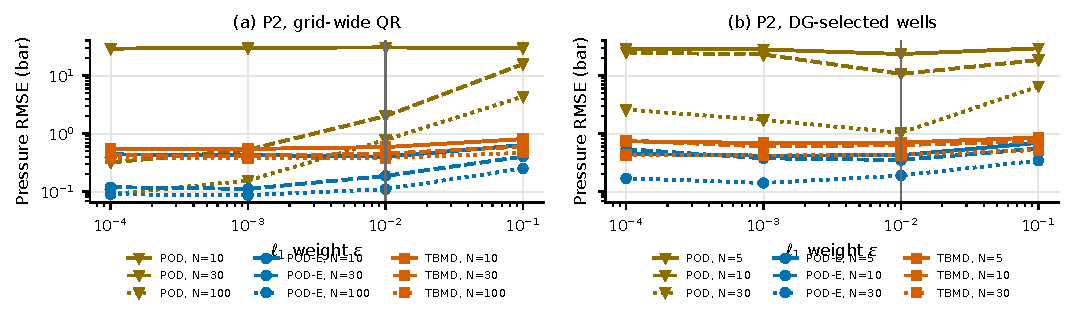
\includegraphics[width=\textwidth]{../../../../studies/brugge_sparse_sensing/figures/figS1_l1_sensitivity.pdf}
\caption{P2 pressure RMSE of the $\ell_1$ estimator against $\varepsilon$ for (a) QR-selected grid channels ($N=10,30,100$) and (b) DG-selected wells ($N=5,10,30$), for POD, POD-E and TBMD $(48,48,2)$ bases. Line style distinguishes budgets; the vertical line marks $\varepsilon=10^{-2}$.}
\label{fig:S_l1}
\end{figure}

\subsection{Example reconstruction}
Figure~\ref{fig:S_maps} shows error maps for one held-out scenario and snapshot.
\begin{figure}[htbp]
\centering
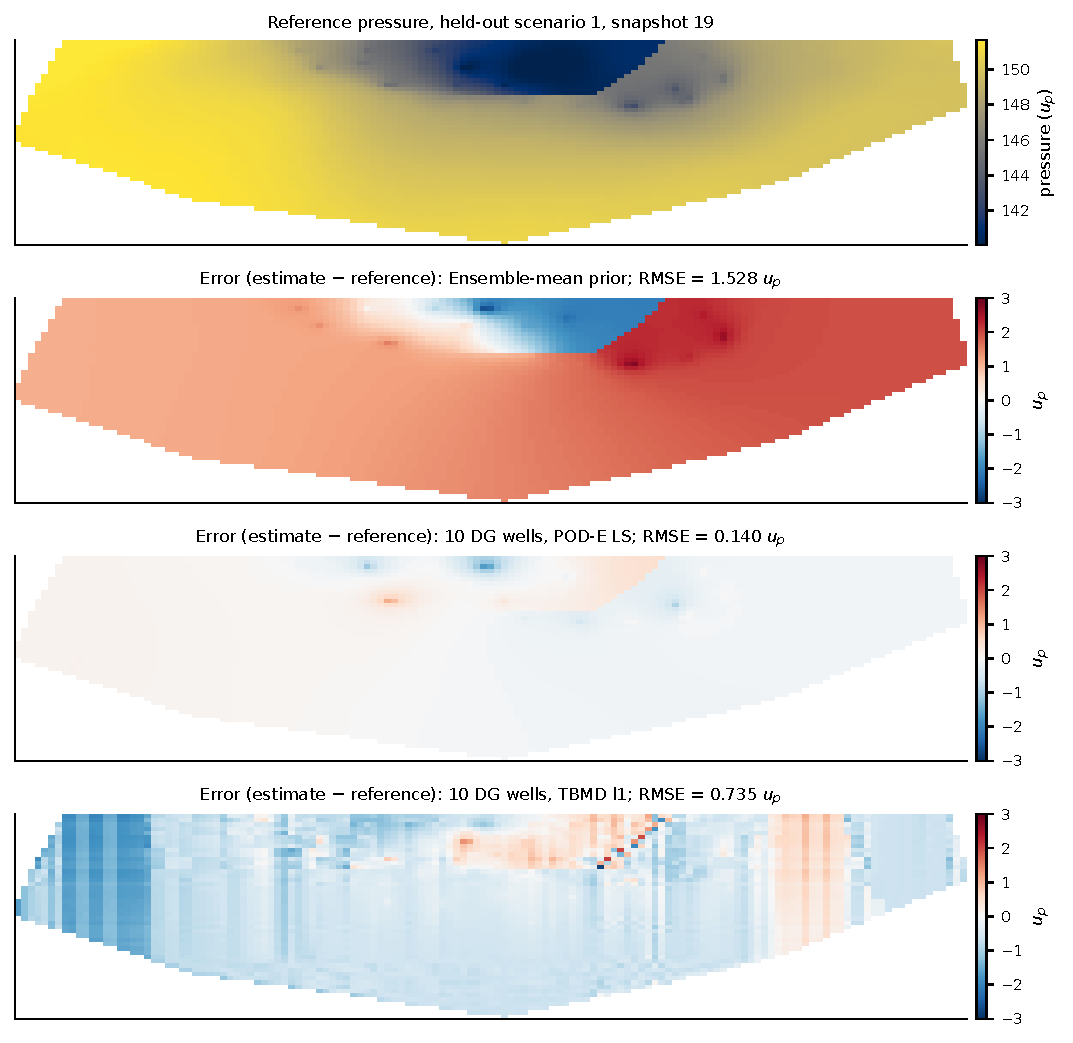
\includegraphics[width=\textwidth]{../../../../studies/brugge_sparse_sensing/figures/figS2_example_maps.pdf}
\caption{Reference pressure of held-out scenario 1 (P2) at the snapshot with the largest cross-scenario spread, and signed errors (estimate minus reference, in $u_p$) of the ensemble-mean prior and of reconstructions from ten DG-selected wells (pressure and $S_o$) with POD-E least squares and with TBMD $(48,48,2)$ $\ell_1$. The panel titles give the RMSE of each map.}
\label{fig:S_maps}
\end{figure}

\subsection{Stability of selections (E5)}
Table~\ref{tab:S_stab} summarises how consistently each basis selects channels and ranks wells across the ten leave-one-out folds.
\begin{table}[htbp]
\centering
\small
\caption{Stability and location of QR selections across the ten P2 leave-one-out bases (\texttt{outputs/e5\_stability.csv}) and Kendall rank correlation of DG well orders.}
\label{tab:S_stab}
\begin{adjustbox}{max width=\linewidth}
\begin{tabular}{@{}lcccccc@{}}
\toprule
Basis & \multicolumn{2}{c}{Mean Jaccard} & \multicolumn{2}{c}{Pressure share (\%)} & Distance to well, $N=50$ & Kendall $\tau$ (wells) \\
 & $N=r$ & $N=50$ & $N=r$ & $N=50$ & (cells) & mean (min) \\
\midrule
POD & \StabJacPodR & \StabJacPodFifty & \StabSharePPodR & \StabSharePPodFifty & \StabDistPodFifty & \StabTauPod{} (\StabTauMinPod) \\
POD-E & \StabJacPodeR & \StabJacPodeFifty & \StabSharePPodeR & \StabSharePPodeFifty & \StabDistPodeFifty & \StabTauPode{} (\StabTauMinPode) \\
TBMD & \StabJacTbmdR & \StabJacTbmdFifty & \StabSharePTbmdR & \StabSharePTbmdFifty & \StabDistTbmdFifty & \StabTauTbmd{} (\StabTauMinTbmd) \\
\bottomrule
\end{tabular}
\end{adjustbox}
\end{table}
The mean distance from an active cell to the nearest well is \StabDistActive{} cells.

\section{Comparison with closest related work}
\label{sec:S_novelty}
\begin{table}[htbp]
\centering
\scriptsize
\caption{Closest related work and differences from this study. Descriptions of prior work are limited to information stated in the cited articles' abstracts or journal records.}
\label{tab:S_novelty}
\begin{tabular}{@{}p{0.15\linewidth}p{0.15\linewidth}p{0.16\linewidth}p{0.13\linewidth}p{0.27\linewidth}@{}}
\toprule
Work & Data & Method / placement & Validation & Difference from this study \\
\midrule
Zhong et al.\ \cite{zhong2024tbmd} & Flow, SST, image data & Third-order Tucker modes; mode-3 fibre QR; $\ell_1$ & vs POD, DMD, POD-based reconstruction & Fourth-order joint-property TBMD; mode-4 fibre QR; property-model and channel ablations; TBMD--POD relation (Prop.~1); references, wells and two protocols \\
Farazmand and Saibaba \cite{farazmand2023} & Kolmogorov flow, SST, 3-D ship flow & Tensor-based reconstruction and placement & vs vectorised methods & On Brugge states, truncated Tucker modes give a floor rather than a gain; storage gain confirmed \\
Zhang et al.\ \cite{zhang2022wind} & 3-D wind fields & Tucker reconstruction; greedy condition-based placement & vs random placement & Confirms that Tucker sparse sensing predates this study outside reservoirs; the present work tests joint properties, well blocks and independent-property controls \\
Manohar et al.\ \cite{manohar2018} & Faces, SST, flows & POD + pivoted QR, LS & vs random sensors & Applied with reservoir wells, IDW and prior references, fold statistics \\
Saito et al.\ \cite{saito2021,saito2020vector} & Synthetic, PIV, climate & POD + determinant greedy (scalar/vector) & accuracy, speed & Block (well) selection vs configured and random orders on reservoir data \\
Peherstorfer et al.\ \cite{peherstorfer2020} & PDE snapshots & DEIM / gappy POD with oversampling & stability analysis & Empirical ill-conditioning with existing wells; $\ell_1$ and energy weighting as remedies \\
Callaham et al.\ \cite{callaham2019} & Flows, geophysical flows & Sparse representation vs LS & noise, corruption & Modal (not example) libraries; $\ell_1$ benefit limited to $m\approx r$ and depends on atom scaling \\
Zou et al.\ \cite{zou2025prosnet} & High-speed-train surface pressure & Neural decoder with differentiable placement & unseen simulated pressure fields & Jointly learns a nonlinear estimator and locations; different domain and data demand, so it is not a fair baseline for the ten-scenario Brugge ensemble \\
Crain et al.\ \cite{crain2023} & CO$_2$ storage models & Monitoring-well optimisation for history matching & synthetic cases & Direct state estimation from point data with learned bases \\
Cardoso and Durlofsky \cite{cardoso2010}; van Doren et al.\ \cite{vandoren2006}; Jansen and Durlofsky \cite{jansen2017rom} & Reservoir simulation & POD-based ROMs & forward prediction, optimisation & No state estimation from sparse measurements \\
\bottomrule
\end{tabular}
\end{table}
The Tucker, QR and sparse-estimation primitives are established. The implementation here is a dimensional generalisation of the published TBMD sensing chain from third- to fourth-order input with an explicit property mode; it does not establish a new decomposition family or priority. The independently assessable contribution is the explicit measurement mapping, the controlled joint-versus-independent property comparison, the separation of energy weighting from spatial truncation, and leakage-controlled reservoir validation. The full text and a reference implementation of Zhong et al.\ were unavailable to this study, so component-level correspondence beyond the publisher-described method is not claimed.

\section{Reproducibility}
\label{sec:S_repro}
All computations are implemented in the study package \texttt{studies/brugge\_sparse\_sensing} of the TBMD repository. The single entry point \texttt{run\_all.sh} executes, in order: input checksums, data manifest (S0), reviewed-configuration provenance (E0), verification against our public library (V1), explicit shape and contraction checks (V3), representation (E1), main benchmark (E2), matched-measurement property coupling (E8), noise (E3), $\ell_1$ sensitivity (E4), ADMM convergence verification (V2), stability (E5), spatial structure (E7), cost (E6), tables, number macros, figures and the consistency check \texttt{check\_claims.py}. Parameters are read from \texttt{config.json}; package versions are pinned in \texttt{requirements-lock.txt}. Random placements use seeds $20260917+s$, $s=0,\dots,19$, and noise draws use $20260917+1000+q$ for fold $q$. Numerical result claims in the main text and Tables~1--2 use generated macros or tables. The macro generator is \texttt{make\_numbers\_tex.py}. The checker requires all canonical macro names and exact non-timing values; only values of existing \texttt{Cost*} timing macros may drift. It also detects result-like decimal literals in the main text.

The working study package includes result files, SHA-256 checksums and independent rerun evidence. Release v2.1.0 predates E8 and V3; the present revision is prepared locally for release as v2.2.0, while tag creation and archival remain external publication actions. Without the input files, \texttt{verify\_outputs.sh} rebuilds tables, Wilcoxon statistics and number macros from stored result files and checks them byte for byte. After a full re-run, \texttt{scripts/compare\_rerun.py} compares every macro and the listed scientific CSVs, including labels and missing-value locations, against the canonical outputs. The independent repeat reproduced non-timing scientific claims; wall-clock measurements varied. These checks do not recover the missing t-Navigator-to-HDF5 export procedure.

E9 has a separate one-command driver, \texttt{run\_e9\_property\_mode.sh}. With \texttt{--full} it validates inputs, rebuilds cross-property diagnostics, executes all inner folds, freezes pairwise common solvers, evaluates every outer fold once, and regenerates E9 tables, figures and macros. Its default \texttt{--reproduce} mode independently refits the frozen selections into a separate output directory and compares every non-runtime outer value to the canonical registry with absolute tolerance $10^{-10}$. The E9 report records the protocol/preregistration hashes and the pre-outer LASSO computational amendment; the independent reproduction validation is \path{outputs/e9_property_mode/reproduction_validation.json}.

\section{Nested optimization details}

\subsection{Search and registry}
For outer scenario $q$, the other nine scenarios are split into three deterministic inner groups. The staged search evaluates representation before sparse sensing, recovery on fixed placement anchors, placement with frozen recovery, and a bounded joint recheck. The resulting files contain \OptValidationRecords{} sparse train-validation rows, \OptOuterRecords{} outer rows and \OptPlacementRecords{} prespecified outer placement-audit rows. Configurations, scenario identifiers, objective values, solver settings and seeds are stored per row; no failed configuration is omitted (none failed in the completed run).

The two final independent-property representations use spatial ranks $(80,48)$ or $(64,48)$ for each property and 16 modal coefficients per property. Scaling is no transform in most folds and RMS scaling in the remainder. Property weights in these independent models algebraically cancel between the per-property fit and expansion and are not interpreted as a source of gain. The joint tensor comparator uses $(80,48,2,32)$ with min--max scaling in every fold.

\subsection{Recovery and placement}
Recovery candidates are minimum-norm LS, relative ridge, L1 ADMM and elastic net. The selected family varies by fold and budget; the complete frozen mapping is in \path{selected_sparse_strategies.json}. Condition-aware, determinant-greedy, configured, whitened-QR, cluster-constrained and well-region placements are all retained in \path{outer_placement_audit.csv}. Random placement uses 20 deterministic orders per fold and is collapsed to one fold median before statistical summaries.

Pressure-objective well order is more stable than joint order (mean Kendall $\tau=\OptWellRankTau$ for condition-aware pressure ranking). The corrected cluster experiment uses active cells only and selects $k$ from train-only silhouette and adjusted-Rand stability. It chooses $k=5$ in every outer-training fit, but does not improve the 30-channel outer benchmark; it becomes competitive only at larger grid budgets.

\subsection{Statistics and reproducibility}
Every table reports ten outer-fold values through mean/standard deviation and median/interquartile summaries. Paired Wilcoxon tests are descriptive because the folds share one fixed-geology ensemble. The generated file \path{paired_statistics.csv} includes raw and Holm-adjusted values; the conservative adjustment covers all comparisons in each metric family, so no broad superiority claim is based on an isolated raw value.

The independent reproduction refits the accuracy TBMD, compression TBMD and POD-E for all outer folds using only frozen JSON selections. All 2,160 identity/configuration records match. Reconstruction metrics agree within absolute tolerance $10^{-10}$ (observed maximum below $3\times10^{-14}$); condition numbers agree within relative tolerance $10^{-12}$. Runtime is excluded from exact equality because it is hardware- and load-dependent.

\subsubsection{Detailed optimization results}


\subsubsection{Representation bottlenecks and train-selected architecture}
The nested study confirms that the original TBMD gap is principally a spatial-truncation floor rather than an unavoidable consequence of tensor representation. At fixed modal depth, inner-validation pressure error falls sharply when $R_2$ reaches the full second grid dimension and continues to improve with $R_1$ (Fig.~\ref{fig:opt_rank}). The original basis has outer full-state pressure/saturation RMSE \OptRepOriginalPressure/\OptRepOriginalSaturation; the train-selected joint $(80,48,2,32)$ basis reaches \OptRepJointPressure/\OptRepJointSaturation. Independent property heads give the lowest equal-property normalized objective, \OptRepAccuracyJoint, while POD-E remains better for pressure alone (\OptRepPodePressure{} versus \OptRepAccuracyPressure). The accuracy and compression TBMD bases store \OptAccuracyCompression{} and \OptCompressionCompression{} times fewer values than rank-32 POD-E (Fig.~\ref{fig:opt_compression}).

\begin{figure}[tbp]
\centering
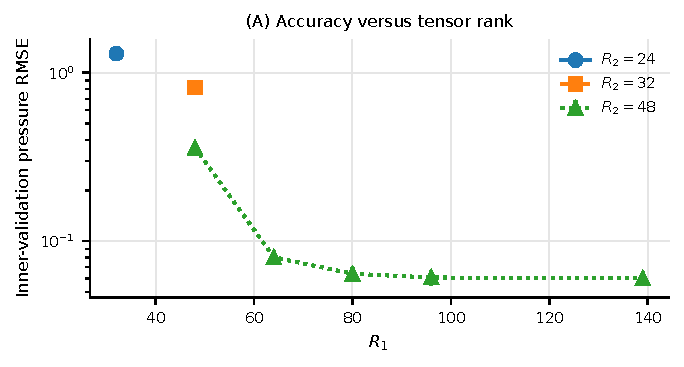
\includegraphics[width=0.62\textwidth]{../../../../studies/brugge_sparse_sensing/figures/fig8_rank_accuracy.pdf}
\caption{Inner-validation pressure RMSE versus spatial tensor ranks at modal rank 16. Error bars show variation across the 30 outer/inner training partitions. The low-$R_2$ configurations are retained as failed accuracy regimes rather than removed from the registry.}
\label{fig:opt_rank}
\end{figure}

\begin{figure}[tbp]
\centering
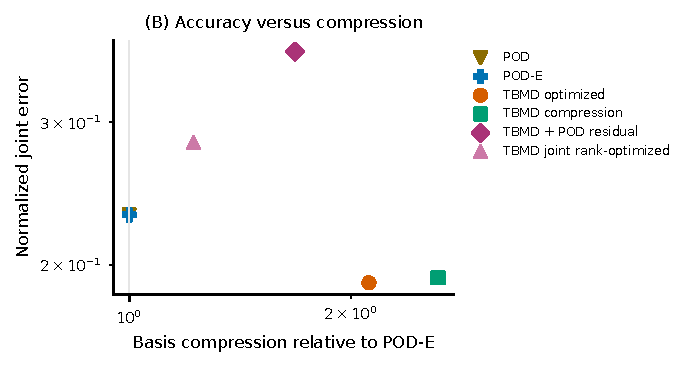
\includegraphics[width=\textwidth]{../../../../studies/brugge_sparse_sensing/figures/fig9_accuracy_compression.pdf}
\caption{Untouched outer full-state normalized joint error versus basis-storage compression relative to POD-E. Pressure and saturation errors are reported separately in the generated tables; the scalar objective does not replace them.}
\label{fig:opt_compression}
\end{figure}

\begin{table*}[t]
\centering
\caption{Evolution of TBMD. Validation gain is relative reduction of the train-only representation objective from the original basis; outer errors use 30 joint wells.}
\label{tab:tbmd_evolution}
\footnotesize
\setlength{\tabcolsep}{2.5pt}
\begin{tabular}{@{}p{0.20\linewidth}p{0.27\linewidth}rrrr@{}}
\toprule
TBMD version & Key change & \shortstack{Validation\\gain} & \shortstack{Pressure\\RMSE ($u_p$)} & \shortstack{$S_o$\\RMSE} & \shortstack{Stored\\floats} \\
\midrule
Original TBMD & Fixed HOOI ranks (48,48,2), fixed L1 & 0.0\% & 0.4323 & 0.004251 & 101.9k \\
Original basis + optimized sensing & Nested placement/recovery & 0.0\% & 0.4289 & 0.004235 & 101.9k \\
Rank-optimized joint TBMD & Spatial/modal rank expansion & 89.8\% & 0.0892 & 0.000643 & 259.2k \\
TBMD + residual & Low-rank POD residual & 86.8\% & 0.2117 & 0.000788 & 188.7k \\
Compressed independent TBMD & Independent properties; 5\% validation tolerance & 93.1\% & 0.1754 & 0.000651 & 120.7k \\
Accuracy-selected independent TBMD & Independent properties; minimum validation loss & 93.2\% & 0.1787 & 0.000644 & 149.7k \\
\bottomrule
\end{tabular}
\end{table*}


\subsubsection{Sparse reconstruction and conditioning}
With joint measurements from all existing wells, POD-E remains the strongest comparator: pressure RMSE is $\OptWellThirtyPodePressure\pm\OptWellThirtyPodePressureSd$, compared with \OptWellThirtyJointPressure{} for rank-optimized joint TBMD and \OptWellThirtyCompressionPressure{} for the compressed independent model (Table~1 of the main manuscript). The original basis remains poor after nested recovery and placement optimization, so recovery alone cannot remove its representation floor. Median budget curves (Fig.~\ref{fig:opt_budget}) also show that placement/regularization transitions can produce non-monotone error; no monotonicity is assumed.

Independent property heads are difficult to observe from joint wells: their block basis has median condition numbers several orders of magnitude above POD-E over much of the budget range (Fig.~\ref{fig:opt_condition}). Ridge, L1 and elastic-net selection controls the resulting variance but does not make conditioning irrelevant. Conversely, pressure-only fitting favours TBMD for pressure (\OptPressureWellThirtyCompressionPressure{} versus \OptPressureWellThirtyPodePressure{} at 30 wells), while its independent saturation head is unobserved. That result is not a joint-state reconstruction advantage.

\begin{figure}[tbp]
\centering
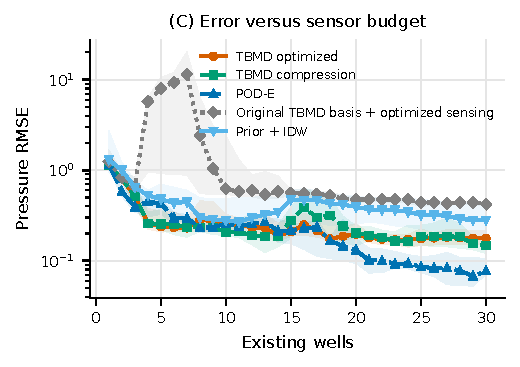
\includegraphics[width=0.62\textwidth]{../../../../studies/brugge_sparse_sensing/figures/fig10_sensor_budget.pdf}
\caption{Median pressure RMSE and interquartile band across outer folds versus the number of existing joint-property wells. Every curve uses parameters selected inside its outer-training partition.}
\label{fig:opt_budget}
\end{figure}

\begin{figure}[tbp]
\centering
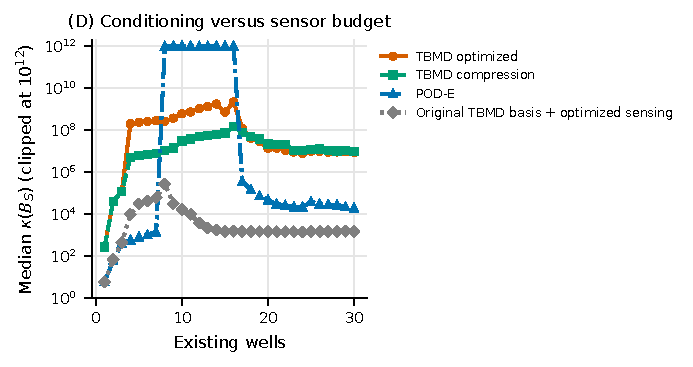
\includegraphics[width=\textwidth]{../../../../studies/brugge_sparse_sensing/figures/fig11_conditioning.pdf}
\caption{Median condition number of the sampled basis versus existing-well budget. Values above $10^{12}$ are clipped only for plotting and remain unmodified in the canonical CSV output.}
\label{fig:opt_condition}
\end{figure}

All-well results are reported in Table~1 of the main manuscript.

\subsubsection{Regime-specific advantage and Pareto decision}
At 100 grid channels, optimized independent TBMD lowers the normalized joint error to \OptGridHundredAccuracyJoint{} from POD-E's \OptGridHundredPodeJoint; at 300 channels the compressed model reaches \OptGridThreeHundredCompressionJoint{} versus \OptGridThreeHundredPodeJoint. The tensor model has higher pressure error but lower saturation error; at 300 channels its joint objective is lower in all ten folds. This identifies a dense-grid, saturation-aware regime rather than universal TBMD superiority.

The ablation (Fig.~\ref{fig:opt_ablation}) attributes the largest gain to correcting tensor ranks. Property separation improves full-state and high-grid-budget joint accuracy, but rank-optimized joint TBMD is better at existing joint wells; the POD-residual hybrid does not supply a consistent additional gain. The Pareto map (the Pareto figure in the main manuscript) therefore supports a regime-specific conclusion: POD-E is preferred for existing joint wells and pressure accuracy, while optimized TBMD occupies the accuracy--storage frontier and can improve the equal-property objective when sufficiently many grid channels observe both properties.

\begin{figure}[tbp]
\centering
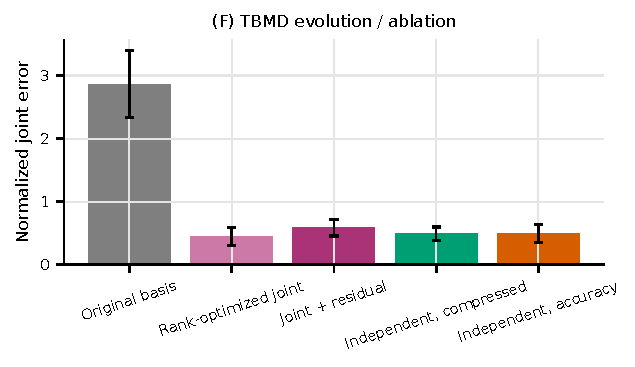
\includegraphics[width=0.68\textwidth]{../../../../studies/brugge_sparse_sensing/figures/fig13_ablation.pdf}
\caption{TBMD evolution/ablation at all 30 joint wells. Bars show mean normalized joint error and error bars show one standard deviation across outer folds.}
\label{fig:opt_ablation}
\end{figure}



\subsubsection{Well ranking and corrected clustering}
Pressure-objective well rankings are stable across folds (mean pairwise Kendall $\tau=\OptWellRankTau$). Early-ranked wells concentrate in regions of higher pressure variability (Fig.~\ref{fig:opt_wells}), but this association is descriptive and does not establish geological causality. The corrected clustering uses active cells only, deterministic seeds, and train-selected silhouette/stability criteria. It selects five clusters in every outer-training fit, but performs poorly at 30 channels and is only competitive at larger budgets. Clustering is therefore retained in the Supplement and registry, not promoted as a main method.

\begin{figure}[tbp]
\centering
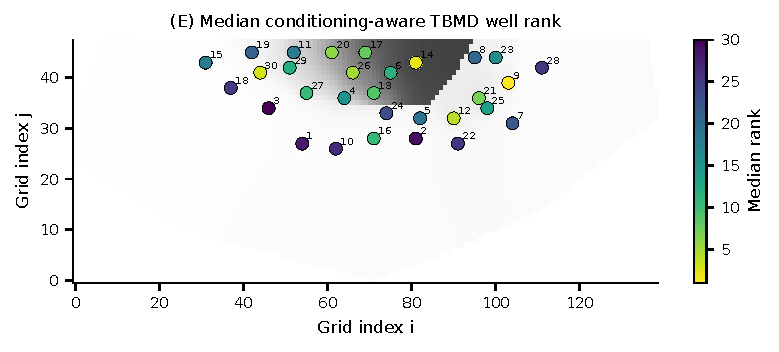
\includegraphics[width=\textwidth]{../../../../studies/brugge_sparse_sensing/figures/fig12_well_ranking.pdf}
\caption{Median conditioning-aware rank of the 30 existing wells for optimized TBMD. Labels are the configured well indices; lower ranks are selected earlier. The background is pressure variability over the supplied ensemble.}
\label{fig:opt_wells}
\end{figure}

\begin{table*}[t]
\centering
\caption{Untouched leave-one-scenario-out reconstruction from all 30 existing wells, with the no-measurement prior shown at zero wells. Values are mean $\pm$ standard deviation across ten outer folds. Bold entries are selected automatically as the smallest column mean.}
\label{tab:optimization_diagnostics}
\resizebox{\textwidth}{!}{%
\begin{tabular}{lrrrrrr}
\toprule
Method & Wells & Pressure RMSE & $S_o$ RMSE & Compression & Storage & Online ms \\
\midrule
POD-E random & 30 & \textbf{0.0840 $\pm$ 0.0273} & \textbf{0.000575 $\pm$ 0.000130} & 1.00$\times$ & 316.8k & -- \\
POD-E & 30 & \textbf{0.0840 $\pm$ 0.0273} & \textbf{0.000575 $\pm$ 0.000130} & 1.00$\times$ & 316.8k & 0.596 \\
TBMD joint rank-optimized & 30 & 0.0892 $\pm$ 0.0234 & 0.000643 $\pm$ 0.000132 & 1.22$\times$ & 259.2k & 1.447 \\
TBMD compression & 30 & 0.1754 $\pm$ 0.0835 & 0.000651 $\pm$ 0.000118 & 2.62$\times$ & 120.7k & 1.476 \\
TBMD optimized & 30 & 0.1787 $\pm$ 0.0463 & 0.000644 $\pm$ 0.000129 & 2.12$\times$ & 149.7k & 1.196 \\
POD & 30 & 0.2164 $\pm$ 0.1231 & 0.000756 $\pm$ 0.000258 & 1.00$\times$ & 316.8k & 0.001 \\
Prior + IDW & 30 & 0.3127 $\pm$ 0.1647 & 0.000780 $\pm$ 0.000197 & -- & 0.0k & -- \\
Original TBMD + tuning & 30 & 0.4289 $\pm$ 0.0506 & 0.004235 $\pm$ 0.000027 & 3.11$\times$ & 101.9k & 0.132 \\
Prior & 0 & 1.1481 $\pm$ 0.5580 & 0.000839 $\pm$ 0.000213 & -- & 0.0k & 0.000 \\
\bottomrule
\end{tabular}
}
\end{table*}


\section{Third- versus fourth-order property-mode experiment (E9)}
\label{sec:S_e9}

\subsection{Frozen protocol and metric correction}
E9 was frozen after the earlier E8 RMSE result was known but before any new E9 outer metric was computed. The preregistration and machine-readable protocol are \path{E9_PREREGISTRATION.md} and \path{studies/brugge_sparse_sensing/e9_protocol.json}; their SHA-256 values are stored in every fold selection record. Ten P2 leave-one-scenario-out folds use three deterministic scenario-grouped inner folds and all 133 report steps only once for the final outer evaluation. Inner selection balances the mean property-wise anomaly-relative error and anomaly DSSIM. The same measurement rows, report steps and one pairwise common inner-selected LS/ridge solver are applied to each 3D--4D comparison. LASSO is a declared frozen-final sensitivity and cannot select a reported model.

\begin{table}[htbp]
\centering
\scriptsize
\caption{Historical metric intent, implementation problem and E9 correction.}
\label{tab:S_e9_metrics}
\begin{tabular}{@{}p{0.22\linewidth}p{0.34\linewidth}p{0.35\linewidth}@{}}
\toprule
Original metric & Audited problem & E9 use \\
\midrule
Relative Frobenius error & Large pressure datum dilutes scenario-specific error; historical call also included inactive cells and rounded estimates & Property-wise physical residual divided by the held-out anomaly norm; raw relative error retained as sensitivity \\
SSIM & Inactive background entered rectangular windows; swapped arguments; non-standard constants; implementation disagreed with the text & Gaussian local moments renormalised over active cells; active-centred windows with at least half active in-domain weight; train-only anomaly range \\
RMSE & Valid physical-unit score but cannot alone compare two differently scaled properties or structure & Mandatory auxiliary endpoint, never removed when it disagrees with anomaly error or SSIM \\
PSNR & Monotone transformation of MSE under fixed range & Omitted \\
\bottomrule
\end{tabular}
\end{table}

Raw-field SSIM is diagnostically saturated: optimized outer records have median scores near one for both properties, while anomaly SSIM spans a broad range and gives materially larger 3D--4D separation. Unit tests establish identity, symmetry, determinism, inactive-background invariance, invalid-window handling, vectorised equivalence and train-only reference fitting.

\subsection{Dependence and property rank}
Figure~\ref{fig:S_e9_coupling} reports dependence using outer-training scenarios only. Cell/time anomalies have correlation \ENineAnomalyCorrelation, but spatial-mean anomaly trajectories correlate at \ENineTemporalCorrelation. Leading spatial subspaces are partly aligned (mean top-16 cosine \ENineSubspaceAlignment) and the leading standardised property direction contains \ENineRankOneEnergy{} of property-mode energy. This combination supports partial sharing and explains why property rank one is not selected. Exploratory fold-level coupling--gain correlations have inconsistent signs across budgets and none survives false-discovery-rate control; they do not establish a causal coupling threshold.

\begin{figure}[htbp]
\centering
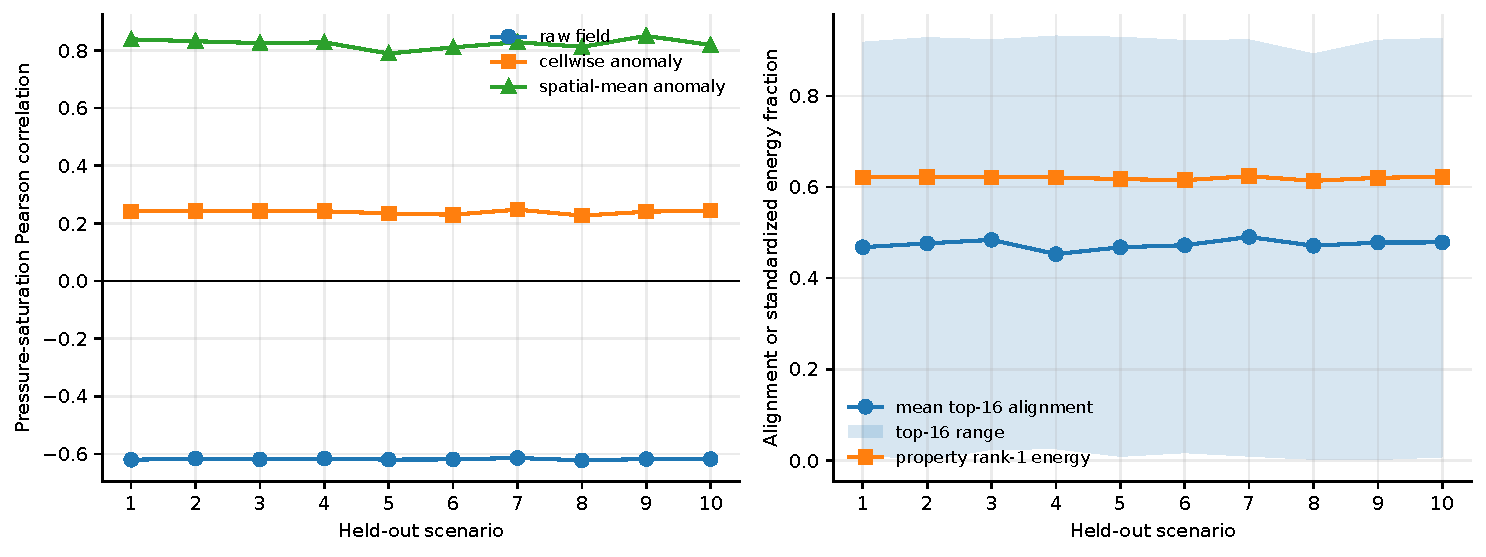
\includegraphics[width=\textwidth]{../../../../studies/brugge_sparse_sensing/figures/fig17_e9_cross_property.pdf}
\caption{Train-only pressure--saturation dependence by held-out scenario. Left: raw, cellwise-anomaly and spatial-mean-anomaly correlations. Right: leading spatial-subspace alignment and the standardised property rank-one energy.}
\label{fig:S_e9_coupling}
\end{figure}

\subsection{Architectures, capacity and ablation}
Independent 3D fits separate space--space--time tensors. 4D-A shares spatial/property factors and coefficients; 4D-B shares spatial factors but not property coefficients; 4D-C weights the joint objective; 4D-D adds property-specific spatial factors; 4D-E adds property-specific tensor residual modes. Equal-total capacity compares 16+16 independent coefficients with 32 fourth-order coefficients; equal-per-property compares 32+32 with 64. Property rank one/two, spatial ranks, anomaly treatment and weighting are selected inside each outer-training fold.

Figure~\ref{fig:S_e9_ablation} reports all fourth-order variants at the prespecified 15-well equal-total slice. Each variant has its own train-only representation and the pairwise common solver selected with independent 3D; the figure does not retrospectively choose the best outer variant. Across the complete selection, 4D-B is chosen in \ENineSharedHeadSelections{} of \ENineSparseSelections{} sparse comparisons and every full-observation comparison. Weighted and residual variants help in individual folds, especially at five wells, but are not stable global winners. The rigid current model meets the headline advantage rule only \ENineCurrentAdvantages{} times; optimization meets it \ENineHeadlineAdvantages{} times out of \ENineHeadlineComparisons.

\begin{figure}[htbp]
\centering
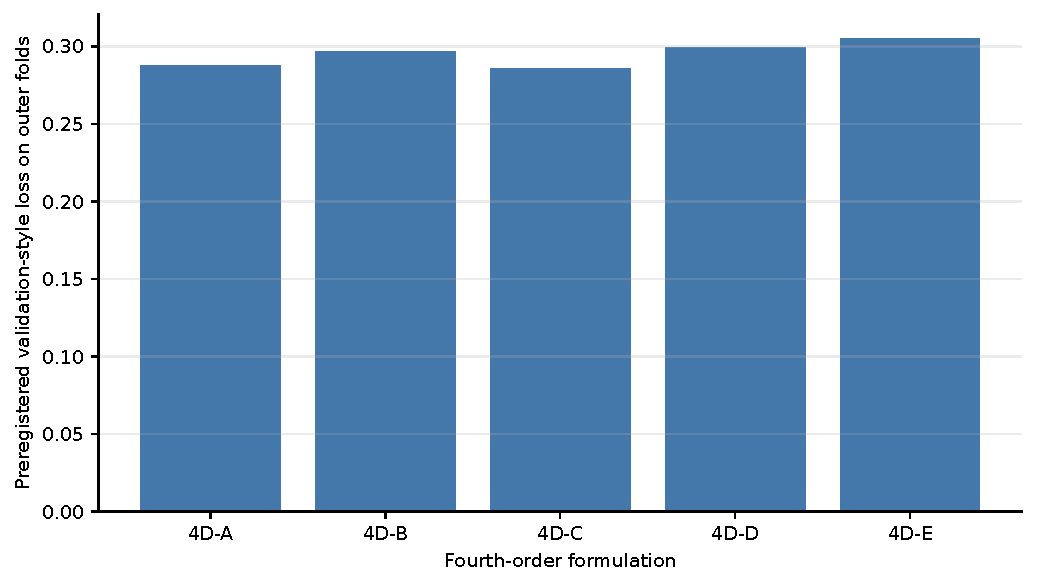
\includegraphics[width=0.82\textwidth]{../../../../studies/brugge_sparse_sensing/figures/fig18_e9_ablation.pdf}
\caption{Fourth-order architecture ablation at 15 configured wells and equal-total capacity. The displayed outer score has the same error/DSSIM form as the frozen validation objective, but outer values never feed selection. Lower is better.}
\label{fig:S_e9_ablation}
\end{figure}

\subsection{Complete evidence and interpretation}
The canonical files \path{outer_selected_results.csv}, \path{outer_summary.csv} and \path{paired_comparisons.csv} contain every fold value, mean, median, SD, IQR, signed paired difference and descriptive Wilcoxon result. \path{selected_configuration_frequency.csv} records fold-specific architectures, transforms, ranks and common solvers. \path{metric_ranking_audit.csv} identifies the \ENineRankingDifferences{} metric-discordant property/regime comparisons rather than collapsing them to one winner. The fixed map metadata are in \path{representative_map_metrics.json}.

The frozen-final LASSO sensitivity contains 320 outer records at the declared $\lambda=10^{-3}$. Raising only the iteration ceiling from 5,000 to 20,000 after the first convergence diagnostic still leaves 50 fits at the ceiling. LASSO favours 4D by the directional fold rule in 49 of 64 regime/metric comparisons, but the unconverged subset makes this supportive rather than confirmatory evidence. No LASSO value enters selection or the headline LS/ridge conclusions; iterations and all failed-to-converge-at-ceiling fits remain visible in \path{lasso_sensitivity.csv}.

The evidence supports shared spatial-factor estimation with independent property heads, especially under severe undersampling. It does not support universal fourth-order superiority, rigid shared coefficients, property rank-one compression, or a full-state saturation gain. E8 therefore remains a valid negative result for the original formulation; E9 explains the limitation and identifies the narrower regime in which a property mode is useful.

% Generated by e9_analyze.py; do not edit.
\begin{table*}[htbp]\centering\small
\caption{E9 equal-total-capacity diagnostic scores and mean factor/core storage (float entries). Pressure RMSE uses the supplied export unit $u_p$; oil-saturation RMSE is dimensionless. Budget counts scalar channels for grid sensing and two-property wells for well sensing. Values are mean $\pm$ sample standard deviation over ten outer scenarios. 3D and 4D denote the independently train-selected models.}
\label{tab:e9_diagnostics}
\setlength{\tabcolsep}{3pt}
\begin{adjustbox}{max width=\textwidth}
\begin{tabular}{lrlrrr}\toprule
Geometry & Budget & Model & RMSE$_p$ & RMSE$_{S_o}$ & Stored floats \\ \midrule
grid & 30 & 3D & 1.166 $\pm$ 0.294 & 0.0008 $\pm$ 0.0003 & 149728 \\
grid & 30 & 4D & 0.372 $\pm$ 0.137 & 0.0004 $\pm$ 0.0001 & 141674 \\
grid & 300 & 3D & 0.147 $\pm$ 0.032 & 0.0003 $\pm$ 0.0001 & 149728 \\
grid & 300 & 4D & 0.102 $\pm$ 0.029 & 0.0003 $\pm$ 0.0001 & 155098 \\
wells & 5 & 3D & 0.486 $\pm$ 0.088 & 0.0018 $\pm$ 0.0002 & 149728 \\
wells & 5 & 4D & 0.411 $\pm$ 0.144 & 0.0009 $\pm$ 0.0002 & 180450 \\
wells & 15 & 3D & 0.210 $\pm$ 0.049 & 0.0010 $\pm$ 0.0002 & 149728 \\
wells & 15 & 4D & 0.216 $\pm$ 0.077 & 0.0008 $\pm$ 0.0003 & 160881 \\
wells & 30 & 3D & 0.189 $\pm$ 0.083 & 0.0007 $\pm$ 0.0002 & 149728 \\
wells & 30 & 4D & 0.121 $\pm$ 0.055 & 0.0007 $\pm$ 0.0003 & 153962 \\
\bottomrule\end{tabular}
\end{adjustbox}
\end{table*}


\subsection{Exact structural metric}
For an active window centre $c$, let $g_{ca}$ be the Gaussian weight of in-domain cell $a$, $m_a$ the binary active mask, and $w_{ca}=g_{ca}m_a/\sum_b g_{cb}m_b$. Windows require $\sum_a g_{ca}m_a/\sum_a g_{ca}\geq 1/2$. For true and reconstructed anomalies $x_a,y_a$, define $\mu_x=\sum_a w_{ca}x_a$, $\mu_y=\sum_a w_{ca}y_a$, $v_x=\max(\sum_a w_{ca}x_a^2-\mu_x^2,0)$, $v_y$ analogously, and $v_{xy}=\sum_a w_{ca}x_ay_a-\mu_x\mu_y$. Then
\begin{equation}
\operatorname{SSIM}'_c=\frac{(2\mu_x\mu_y+C_1)(2v_{xy}+C_2)}{(\mu_x^2+\mu_y^2+C_1)(v_x+v_y+C_2)},\qquad C_j=(K_j L_k)^2.
\label{eq:S_ssim}
\end{equation}
Here $L_k$ is the training-anomaly range for property $k$, $K_1=0.01$ and $K_2=0.03$. Equation~\eqref{eq:S_ssim} uses population moments; no sample-covariance correction is applied. Zero padding carries zero domain weight. The implementation averages valid centres and report steps equally. A zero anomaly range falls back to the raw training range; a zero raw range is rejected. A zero anomaly-error denominator gives zero only for exact reconstruction and infinity otherwise. None of these degenerate cases occurs in the retained outer results.

\section{Fixed-rank benchmark: complete results}
\label{sec:S_legacy}

\subsection{Experiment inventory}

\begin{itemize}
\item \textbf{V1 (extension verification):} fourth-order QR pivots and $\ell_1$ reconstruction are compared with the public TBMD library; the untruncated TBMD--POD-E identity is checked numerically (RQs 1--2).
\item \textbf{E0 (lineage):} re-execution of the archived notebook configuration (Supplementary Section~S2).
\item \textbf{E1 (representation):} full-observation least-squares projection of held-out snapshots onto POD and TBMD for $r\in\{2,\allowbreak 5,\allowbreak 10,\allowbreak 16,\allowbreak 20,\allowbreak 30,\allowbreak 50\}$ and the training-selected depth, and onto TBMD with $R_1\in\{12,\allowbreak 24,\allowbreak 48,\allowbreak 96,\allowbreak 139\}$, $R_2=\min(R_1,48)$, at the selected depth (RQ2).
\item \textbf{E2 (main benchmark):} bases \{POD, POD-E, TBMD\} $\times$ placements \{QR/DG on the same basis, configured order, 20 random orders\} $\times$ estimators \{LS, $\ell_1$\}, plus prior and prior + IDW; 12 grid-wide budgets of 2--300 channels and 10 well budgets of 1--30 wells, with joint (pressure and $S_o$) or pressure-only well sensors; both protocols, all ten folds (RQs 1, 3, 4).
\item \textbf{E3 (noise):} P2, DG-selected wells ($N=10,30$), grid-wide QR ($N=30$) and configured order; five Gaussian-noise levels, ten draws per level (RQ5; Supplementary Section~S3).
\item \textbf{E4 ($\ell_1$ weight):} P2, $\varepsilon\in\{10^{-4},10^{-3},10^{-2},10^{-1}\}$ for QR ($N=10,30,100$) and DG wells ($N=5,10,30$) (RQ5).
\item \textbf{E5 (stability and interpretation):} Jaccard similarity of QR selections and Kendall rank correlation of DG well orders across the ten P2 bases; comparison of selected cells with the training temporal standard deviation and the distance to existing wells (RQ5).
\item \textbf{E6 (cost):} single-thread wall time of offline (SVD, Tucker, QR, DG) and online (per-snapshot LS and $\ell_1$) steps, median of repeated runs (RQ5).
\item \textbf{E8 (property coupling):} joint fourth-order versus independent third-order TBMD, identical folds and measurements at 10 or 30 configured wells, matched total or per-property coefficient counts, LS and $\ell_1$ (RQ2; Supplementary Section~S4).
\item \textbf{E9 (third versus fourth order):} a frozen nested comparison of independent third-order TBMD with five fourth-order coupling architectures under equal-total and equal-per-property capacities; full observation, 5--30 configured wells and 30--300 common grid channels; property-wise reconstruction error, mask-aware SSIM and RMSE; all ten P2 outer folds (RQ6; the main manuscript). E9 supersedes E8 for the dimensionality question but retains E8 as provenance for the original rigid formulation.
\item \textbf{O1--O5 (nested optimization):} train-only representation search; recovery tuning; placement tuning; bounded joint refinement; one outer evaluation; prespecified placement audit; and independent frozen refitting. The registry contains \OptValidationRecords{} sparse validation records and \OptOuterRecords{} outer records (RQs 1--5; the main manuscript).
\end{itemize}


\subsection{References without measurements and the choice of protocol}
\label{sec:res_protocol}
The field-mean pressure of all scenarios falls during early production, recovers and then varies slowly (Fig.~\ref{fig:data}a). The scenarios differ by a persistent pressure deviation whose cross-scenario standard deviation, averaged over cells, peaks at \CrossSdMax{} $u_p$ and is \CrossSdEnd{} $u_p$ at the last snapshot (Fig.~\ref{fig:data}b). Over the P1 hold-out window, persistence of the last training snapshot has a pressure RMSE that grows from \PersistFirst{} $u_p$ at the first held-out snapshot to \PersistLast{} $u_p$ at the last one. Averaged over the window and the ten scenarios, persistence reaches $\mathrm{RMSE}_p=\POnePriorGridTenP\pm\POnePriorGridTenPsd\,u_p$ and $\mathrm{RMSE}_{S_o}=\POnePriorGridTenS\times10^{-3}$ (Table~\ref{tab:S_P1}). In P2, the ensemble mean of the other scenarios reaches $\PTwoPriorGridTenP\pm\PTwoPriorGridTenPsd\,u_p$ and $\PTwoPriorGridTenS\times10^{-3}$. Saturation differences between scenarios are therefore very small. Because persistence is already accurate in P1, the main comparisons use P2.

\begin{figure}[tbp]
\centering
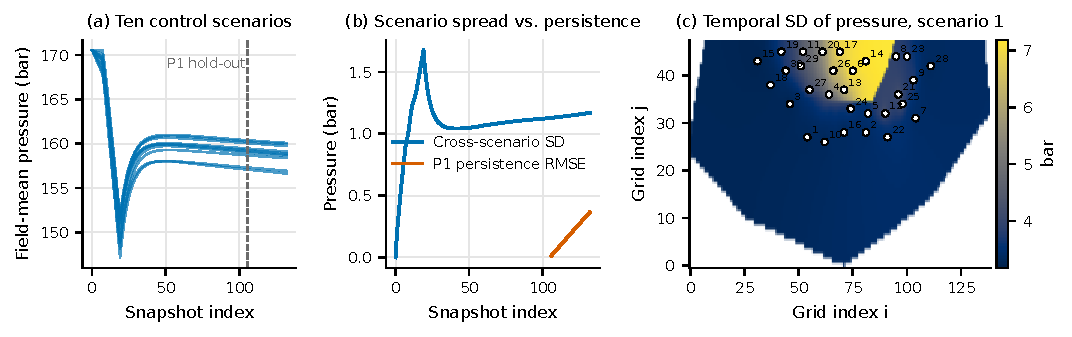
\includegraphics[width=\textwidth]{../../../../studies/brugge_sparse_sensing/figures/fig2_data_context.pdf}
\caption{Brugge control ensemble used in this study. (a) Field-mean pressure (supplied export unit $u_p$) of the ten control scenarios against snapshot index; the dashed line marks the start of the P1 hold-out window. (b) Cross-scenario standard deviation of pressure, averaged over active cells, and pressure RMSE of persistence of the last training snapshot over the P1 window (mean over scenarios). (c) Temporal standard deviation of pressure in scenario~1 on the $139\times48$ grid (inactive cells blank), with the 30 existing wells labelled by their configured order.}
\label{fig:data}
\end{figure}


\subsection{Representation capacity of the bases (RQ1)}
\label{sec:res_representation}
The energy criterion selects $r=\RankPTwoMin$ in every P2 fold and $r\in\{\RankPOneMin,\RankPOneMax\}$ in P1. With all active channels observed, the POD and POD-E bases (which share a subspace) reproduce held-out P2 states with $\mathrm{RMSE}_p=\EOnePTwoPodOracle\,u_p$, while TBMD with $(R_1,R_2,R_3)=(48,48,2)$ reaches only \EOnePTwoTbmdOracle{} $u_p$ at the same depth (Fig.~\ref{fig:representation}a,b). This TBMD floor is about \EOnePTwoFloorRatio{} times the POD error and does not decrease with depth, because it is set by the spatial truncation (Fig.~\ref{fig:representation}c). The TBMD error decreases monotonically with $R_1$ and coincides with POD at $R_1=139$, as Proposition~1 of the main manuscript predicts; numerically, the relative difference of the singular values and the subspace distance are both below \PropSvDiff{}. In P1 the TBMD floor (\EOnePOneTbmdOracle{} $u_p$) already exceeds the error of persistence (\POnePriorGridTenP{} $u_p$); consistently, no TBMD configuration in P1 improved on persistence (best mean error \POneTbmdBest{} $u_p$; Supplementary Table~S3).

\begin{figure}[tbp]
\centering
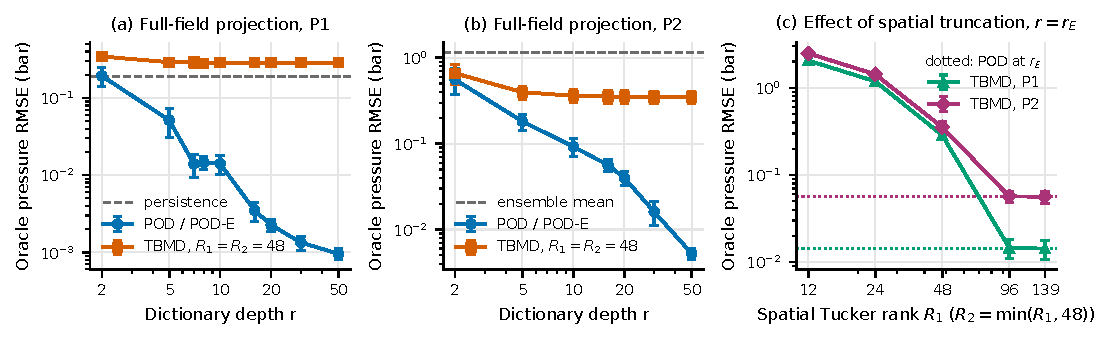
\includegraphics[width=\textwidth]{../../../../studies/brugge_sparse_sensing/figures/fig3_representation.pdf}
\caption{Representation capacity with all active channels observed (least-squares projection of held-out snapshots). (a, b) Pressure RMSE against dictionary depth $r$ for POD/POD-E (identical subspace) and TBMD with spatial ranks $(48,48,2)$ in P1 and P2; dashed line: no-measurement reference. (c) TBMD pressure RMSE against the spatial Tucker rank $R_1$ ($R_2=\min(R_1,48)$, $R_3=2$) at the training-selected depth; dotted lines: POD at the same depth. Markers: mean over ten folds; bars: one standard deviation.}
\label{fig:representation}
\end{figure}


\subsection{Grid-wide sensing (RQs 3 and 5)}
\label{sec:res_grid}
Figure~\ref{fig:budget}a and Table~\ref{tab:main} show three regimes for grid-wide channels in P2.
\emph{Below the depth ($N<r$)} the orthonormal POD basis fails: with $N=10$ QR-selected channels, POD gives $\PTwoPodLsGridTenP\,u_p$ with LS and $\PTwoPodLoneGridTenP\,u_p$ with $\ell_1$. The energy-weighted bases remain below the prior. POD-E with LS gives $(\PTwoPodeLsGridTenP\pm\PTwoPodeLsGridTenPsd)\,u_p$ (better than POD LS in \WPTwoPodELsVsPodLsGridTenWins{} of 10 folds, $p=\WPTwoPodELsVsPodLsGridTen$), and TBMD with $\ell_1$ gives $(\PTwoTbmdLoneGridTenP\pm\PTwoTbmdLoneGridTenPsd)\,u_p$.
\emph{At and above the depth} POD and POD-E agree for the same measurement rows when the sampled basis has full column rank; their separately optimised placements need not coincide. With $N=30$ channels the error is $(\PTwoPodeLsGridThirtyP\pm\PTwoPodeLsGridThirtyPsd)\,u_p$, a factor of about \PTwoGainPriorGridThirty{} below the prior. POD-E LS is lower than prior + IDW ($\PTwoIdwGridThirtyP\,u_p$) and than the original TBMD configuration ($\PTwoTbmdLoneGridThirtyP\,u_p$) in \WPTwoQrPodELsVsIdwGridThirtyWins{} and \WPTwoQrPodELsVsQrTbmdLGridThirtyWins{} of 10 folds, respectively ($p=\WPTwoQrPodELsVsIdwGridThirty$ in both cases). With $N=100$ channels POD-E LS reaches $\PTwoPodeLsGridHundredP\,u_p$, whereas TBMD saturates at $\PTwoTbmdLoneGridHundredP\,u_p$, close to its representation floor.
\emph{Placement} matters. At $N=30$, QR-selected channels give a lower error than the median of 20 random selections in \WPTwoQrPodELsVsRandomMedianGridThirtyWins{} of 10 folds ($p=\WPTwoQrPodELsVsRandomMedianGridThirty$; random median $\PTwoRandLsGridThirtyP\,u_p$). At $N=10$ they are better in \WPTwoQrPodELsVsRandomMedianGridTenWins{} folds ($p=\WPTwoQrPodELsVsRandomMedianGridTen$).
Saturation errors change little: POD-E LS gives $\PTwoPodeLsGridHundredS\times10^{-3}$ at $N=100$ against $\PTwoPriorGridTenS\times10^{-3}$ for the prior, and prior + IDW increases the saturation error (Supplementary Table~S4).

\begin{figure}[tbp]
\centering
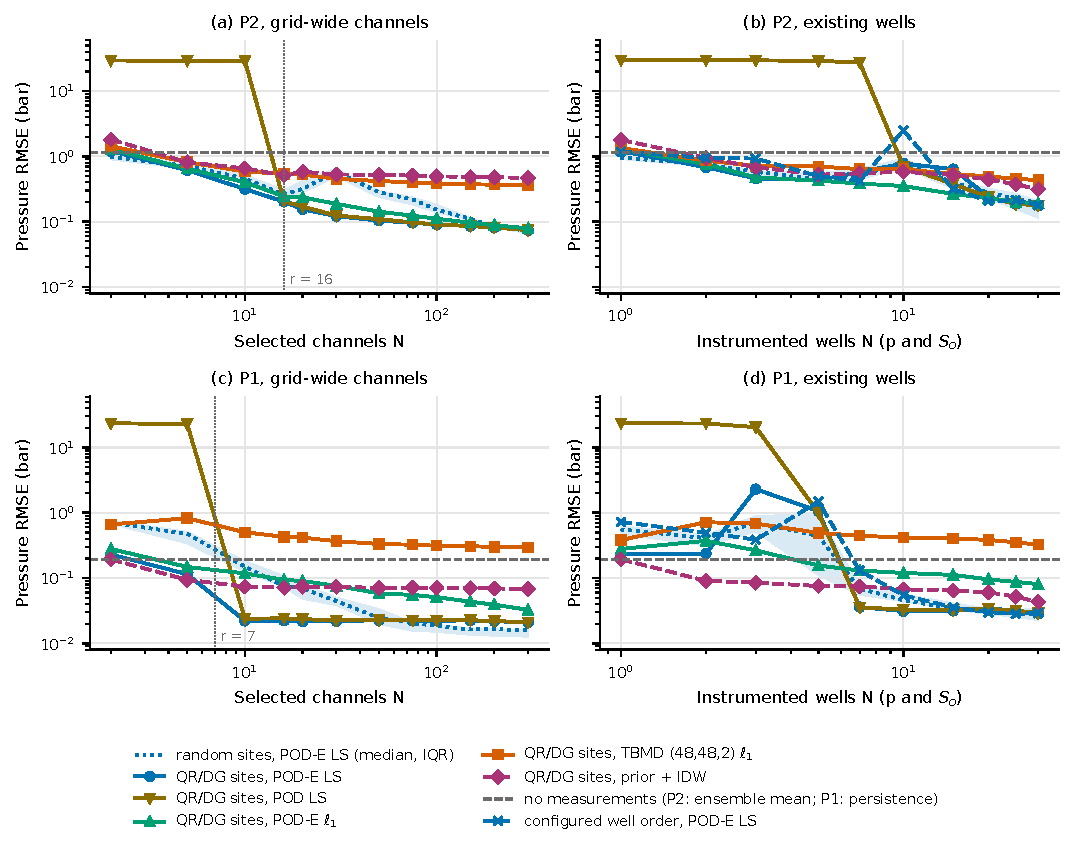
\includegraphics[width=\textwidth]{../../../../studies/brugge_sparse_sensing/figures/fig4_budget_curves.pdf}
\caption{Pressure RMSE (supplied export unit $u_p$; mean over ten folds) against the measurement budget. (a) P2, grid-wide channels; (b) P2, existing wells measuring pressure and $S_o$; (c, d) the same for P1. QR: pivoted-QR/determinant-greedy channels; DG: determinant-greedy well order; both computed on the basis named in the legend. The shaded band and dotted line show the interquartile range and median over folds of the per-fold median of 20 random placements (POD-E, LS). Dashed grey: no-measurement reference; vertical dotted line: dictionary depth $r$. Axes are logarithmic; standard deviations are given in Table~\ref{tab:main}.}
\label{fig:budget}
\end{figure}

\begin{table}[tbp]
\centering
\scriptsize
\setlength{\tabcolsep}{2.5pt}
\caption{Pressure RMSE (bar) in protocol P2, mean\,$\pm$\,standard deviation over the ten held-out control scenarios. Placement is QR (grid) or DG (wells) on the basis of the same row unless stated; $r=16$ in every fold. The prior row uses no measurements and is repeated across columns. Random: per-fold median over 20 placements.}
\label{tab:main}
\begin{tabular}{@{}lcccccc@{}}
\toprule
 & \multicolumn{3}{c}{Grid-wide channels} & \multicolumn{2}{c}{Wells ($p$, $S_o$)} & Wells ($p$) \\
\cmidrule(lr){2-4}\cmidrule(lr){5-6}\cmidrule(l){7-7}
Method & $N=10$ & $N=30$ & $N=100$ & $N=10$ & $N=30$ & $N=30$ \\
\midrule
No measurements (prior) & 1.15\,$\pm$\,0.56 & 1.15\,$\pm$\,0.56 & 1.15\,$\pm$\,0.56 & 1.15\,$\pm$\,0.56 & 1.15\,$\pm$\,0.56 & 1.15\,$\pm$\,0.56 \\
Prior + IDW (POD-E sites) & 0.65\,$\pm$\,0.35 & 0.53\,$\pm$\,0.27 & 0.50\,$\pm$\,0.26 & 0.58\,$\pm$\,0.24 & 0.31\,$\pm$\,0.16 & 0.31\,$\pm$\,0.16 \\
POD, LS & 29\,$\pm$\,1 & 0.12\,$\pm$\,0.04 & 0.09\,$\pm$\,0.02 & 0.70\,$\pm$\,0.30 & 0.18\,$\pm$\,0.09 & 0.23\,$\pm$\,0.09 \\
POD, $\ell_1$ & 31\,$\pm$\,1 & 2.01\,$\pm$\,0.27 & 0.78\,$\pm$\,0.13 & 11\,$\pm$\,3 & 1.04\,$\pm$\,0.24 & 5.04\,$\pm$\,0.70 \\
POD-E, LS & 0.32\,$\pm$\,0.18 & 0.12\,$\pm$\,0.04 & 0.09\,$\pm$\,0.02 & 0.78\,$\pm$\,0.45 & 0.18\,$\pm$\,0.09 & 0.23\,$\pm$\,0.09 \\
POD-E, $\ell_1$ & 0.40\,$\pm$\,0.18 & 0.19\,$\pm$\,0.03 & 0.11\,$\pm$\,0.02 & 0.35\,$\pm$\,0.10 & 0.19\,$\pm$\,0.03 & 0.21\,$\pm$\,0.08 \\
TBMD $(48,48,2)$, LS & 0.54\,$\pm$\,0.08 & 0.42\,$\pm$\,0.06 & 0.38\,$\pm$\,0.06 & 1.27\,$\pm$\,0.38 & 0.43\,$\pm$\,0.05 & 0.48\,$\pm$\,0.05 \\
TBMD $(48,48,2)$, $\ell_1$ & 0.59\,$\pm$\,0.12 & 0.45\,$\pm$\,0.07 & 0.38\,$\pm$\,0.06 & 0.64\,$\pm$\,0.13 & 0.43\,$\pm$\,0.06 & 0.43\,$\pm$\,0.06 \\
Random sites, POD-E, LS & 0.45\,$\pm$\,0.12 & 0.59\,$\pm$\,0.13 & 0.16\,$\pm$\,0.03 & 0.84\,$\pm$\,0.27 & 0.18\,$\pm$\,0.09 & 0.23\,$\pm$\,0.09 \\
Configured wells, POD-E, LS & -- & -- & -- & 2.50\,$\pm$\,1.55 & 0.18\,$\pm$\,0.09 & 0.23\,$\pm$\,0.09 \\
Configured wells, TBMD, $\ell_1$ & -- & -- & -- & 0.47\,$\pm$\,0.07 & 0.43\,$\pm$\,0.06 & 0.43\,$\pm$\,0.06 \\
\bottomrule
\end{tabular}
\end{table}


\subsection{Existing wells (RQs 3--4)}
\label{sec:res_wells}
With measurements restricted to the \NWells{} existing wells, each contributing pressure and $S_o$ (Fig.~\ref{fig:budget}b), prior + IDW is a strong reference: with all wells it reaches $(\PTwoIdwWellThirtyP\pm\PTwoIdwWellThirtyPsd)\,u_p$ and is better than the prior in \WPTwoIdwVsPriorWellsJointThirtyWins{} of 10 folds. With all 30 wells, POD-E gives $(\PTwoPodeLsWellThirtyP\pm\PTwoPodeLsWellThirtyPsd)\,u_p$ with LS and $(\PTwoPodeLoneWellThirtyP\pm\PTwoPodeLoneWellThirtyPsd)\,u_p$ with $\ell_1$. The $\ell_1$ estimate is better than prior + IDW in \WPTwoPodELVsIdwWellsJointThirtyWins{} of 10 folds ($p=\WPTwoPodELVsIdwWellsJointThirty$); the LS estimate only in \WPTwoPodELsVsIdwWellsJointThirtyWins{} ($p=\WPTwoPodELsVsIdwWellsJointThirty$). Both are better than the original TBMD configuration ($\PTwoTbmdLoneWellThirtyP\,u_p$) in all folds.

With ten wells (20 channels for $r=\RankPTwoMin$) the least-squares problem is poorly conditioned \cite{peherstorfer2020}: the median condition number of the sensing matrix is \CondDgTen{} for DG-selected wells, \CondRandTen{} for random wells and \CondConfTen{} for the configured order, against \CondDgThirty{} with all 30 wells. POD-E LS gives $(\PTwoPodeLsWellTenP\pm\PTwoPodeLsWellTenPsd)\,u_p$ with DG-selected wells and $(\PTwoConfLsWellTenP\pm\PTwoConfLsWellTenPsd)\,u_p$ with the configured order. DG ordering is better than the configured order in \WPTwoDgVsConfiguredPodELsWellsJointTenWins{} of 10 folds ($p=\WPTwoDgVsConfiguredPodELsWellsJointTen$), but LS is not consistently better than the prior (\WPTwoPodELsVsPriorWellsJointTenWins{} of 10 folds). The $\ell_1$ estimator on POD-E removes this instability: $(\PTwoPodeLoneWellTenP\pm\PTwoPodeLoneWellTenPsd)\,u_p$, better than the prior in \WPTwoPodELVsPriorWellsJointTenWins{}, than prior + IDW in \WPTwoPodELVsIdwWellsJointTenWins{} ($p=\WPTwoPodELVsIdwWellsJointTen$) and than TBMD $\ell_1$ in \WPTwoPodELVsTbmdLWellsJointTenWins{} of 10 folds. With $\ell_1$ the well order matters little: \LoneDgTen{} $u_p$ (DG), \LoneConfTen{} $u_p$ (configured) and \LoneRandTen{} $u_p$ (median of random orders).

Pressure-only gauges at all 30 wells give $\PTwoPodeLsPWellThirtyP\,u_p$ with POD-E LS, close to joint sensing, so the saturation channel adds little to pressure reconstruction. Inferring $S_o$ from pressure through the joint basis, however, increases the saturation error by more than an order of magnitude ($\PTwoPodeLsPWellThirtyS\times10^{-3}$ against $\PTwoPriorGridTenS\times10^{-3}$; Supplementary Table~S4). Joint well measurements reduce the saturation error relative to the prior in \WPTwoPodELsVsPriorSoWellsJointThirtyWins{} of 10 folds ($p=\WPTwoPodELsVsPriorSoWellsJointThirty$), i.e. not consistently.

Figure~\ref{fig:time} resolves the P2 errors in time for ten DG-selected wells. At the first snapshot all scenarios share the initial state, so the prior and prior + IDW are exact, whereas POD-E $\ell_1$ has a median error of \TimeLoneFirst{} $u_p$. From snapshot \TimeCrossover{} onwards the POD-E $\ell_1$ error stays below the prior error. Its median error is \TimeLoneEarly{} $u_p$ over snapshots 0--30, which include the production transient, and \TimeLoneLate{} $u_p$ afterwards; the prior gives \TimePriorEarly{} and \TimePriorLate{} $u_p$ over the same periods.

\begin{figure}[tbp]
\centering
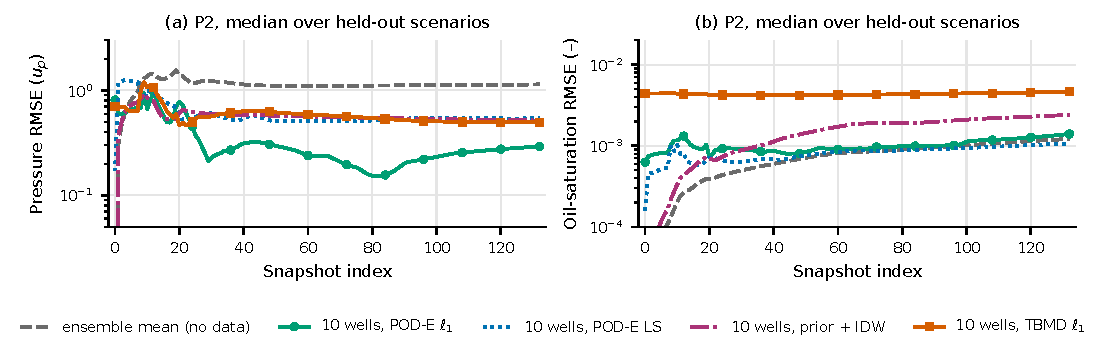
\includegraphics[width=\textwidth]{../../../../studies/brugge_sparse_sensing/figures/fig5_time_resolved.pdf}
\caption{Time-resolved errors in P2 for ten DG-selected wells measuring pressure and $S_o$: median over the ten held-out scenarios of (a) pressure RMSE and (b) oil-saturation RMSE at each snapshot, for the ensemble-mean prior, prior + IDW, POD-E with $\ell_1$ and with least squares, and TBMD $(48,48,2)$ with $\ell_1$.}
\label{fig:time}
\end{figure}


\subsection{Robustness, stability and cost (RQs 3--5)}
\label{sec:res_robust}
\textbf{Noise.} Figure~\ref{fig:noise} shows that least squares with ten wells amplifies measurement noise strongly: POD-E LS rises to \NoiseWellTenPodeLsSigOne{} $u_p$ at $\sigma_p=1\,u_p$, whereas POD-E $\ell_1$ gives \NoiseWellTenPodeLoneSigOne{} $u_p$ and prior + IDW \NoiseWellTenIdwSigOne{} $u_p$. With 30 wells the difference is smaller: \NoiseWellThirtyPodeLsSigOne{} $u_p$ for LS, \NoiseWellThirtyPodeLoneSigOne{} $u_p$ for $\ell_1$ and \NoiseWellThirtyIdwSigOne{} $u_p$ for IDW at $\sigma_p=1\,u_p$. At $\sigma_p=2\,u_p$ the $\ell_1$ and IDW errors are close to the prior error with ten wells (\NoiseWellTenPodeLoneSigTwo{} and \NoiseWellTenIdwSigTwo{} $u_p$) and below it with 30 wells (\NoiseWellThirtyPodeLoneSigTwo{} and \NoiseWellThirtyIdwSigTwo{} $u_p$), whereas least squares exceeds the prior error in both cases (\NoiseWellTenPodeLsSigTwo{} and \NoiseWellThirtyPodeLsSigTwo{} $u_p$).

\textbf{$\ell_1$ weight.} POD-E and TBMD change moderately for $\varepsilon=10^{-4}$--$10^{-2}$ and worsen at $10^{-1}$. Orthogonal POD fails below the depth for every tested weight because its coefficients are large relative to the penalty (Supplementary Fig.~S1). Although $\varepsilon=10^{-3}$ lowers POD-E error in four of six designs, we retain the fixed $10^{-2}$ value because that observation used held-out scenarios; retuning would require a separate validation split.

\textbf{Stability and interpretation.} QR selections for POD-E at $N=50$ overlap between leave-one-out bases with a mean Jaccard index of \StabJacPodeFifty{}, and \StabSharePPodeFifty{}\,\% of the selected channels are pressure channels. On average, the selected cells lie at percentile \StabTstdPodeFifty{} of the training temporal standard deviation of the measured property, and their mean distance to the nearest existing well is \StabDistPodeFifty{} cells, against \StabDistActive{} cells over all active cells; the placement therefore concentrates on dynamically active regions around wells (Fig.~\ref{fig:maps}a). DG rankings of existing wells are consistent across folds (mean Kendall $\tau=\StabTauPode$; Fig.~\ref{fig:maps}b).

\textbf{Cost.} On one CPU thread (P2, $r=16$, \NT{}$\times$9 training snapshots), the POD basis takes \CostPodSvd{} s and the Tucker model \CostTucker{} s. TBMD-based QR placement of $r$ sensors takes \CostQr{} ms and DG ranking of 30 wells \CostBlockDg{} ms. Online POD-E coefficient estimation from 30 wells takes \CostLsWell{}\,\si{\micro\second} with LS and \CostLoneWell{}\,\si{\micro\second} with ADMM per snapshot (fold-amortised, excluding full-state synthesis and inverse scaling; Table~\ref{tab:cost}). The TBMD factors store \TbmdStorage{} numbers against \BasisStorage{} for an explicit basis matrix.

\begin{figure}[tbp]
\centering
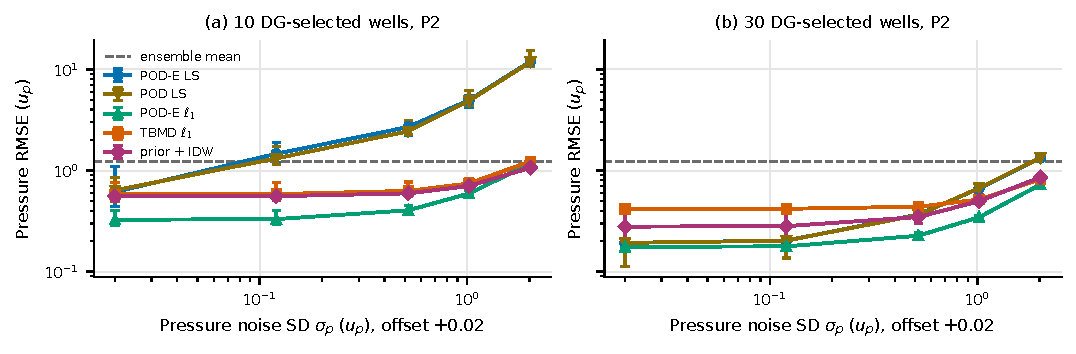
\includegraphics[width=\textwidth]{../../../../studies/brugge_sparse_sensing/figures/fig6_noise.pdf}
\caption{Effect of measurement noise in P2 for (a) 10 and (b) 30 DG-selected wells measuring pressure and $S_o$. Noise standard deviations are $(\sigma_p,\sigma_{S_o})\in\{(0,0),(0.1,0.005),(0.5,0.01),(1,0.02),(2,0.05)\}$ in ($u_p$, dimensionless); the horizontal axis shows $\sigma_p+0.02\,u_p$ so that the noise-free case appears on the logarithmic axis. Markers: median over folds of the per-fold mean over ten noise draws (one evaluation at zero noise); bars: interquartile range over folds; dashed grey: ensemble-mean prior.}
\label{fig:noise}
\end{figure}

\begin{figure}[tbp]
\centering
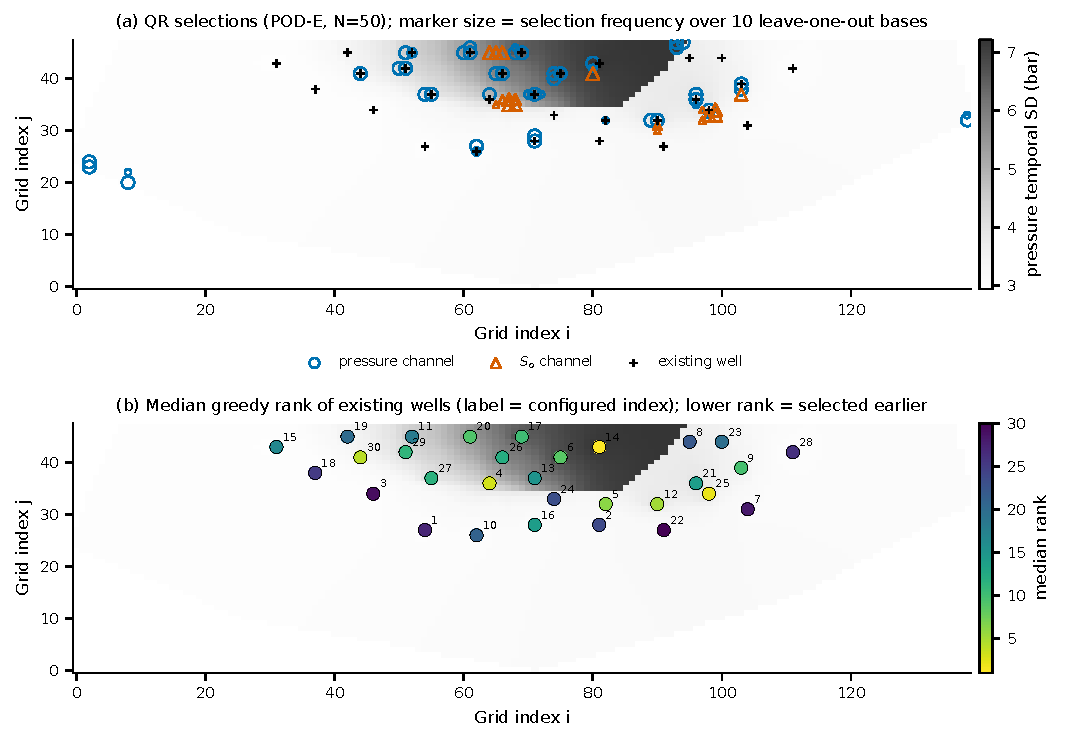
\includegraphics[width=\textwidth]{../../../../studies/brugge_sparse_sensing/figures/fig7_sensor_maps.pdf}
\caption{Location of selected sensors in P2. (a) QR selections on POD-E for $N=50$ channels; marker size is the fraction of the ten leave-one-out bases in which a channel was selected (circles: pressure; triangles: $S_o$); background: temporal standard deviation of pressure averaged over all ten scenarios (descriptive background only); crosses: existing wells. (b) Median DG rank of each existing well over the ten folds (colour; rank 1 is selected first), labelled by configured order.}
\label{fig:maps}
\end{figure}

\begin{table}[tbp]
\centering
\small
\caption{Single-thread wall time (median of repeated runs) for P2 fold 1; online times are per snapshot, amortised over the 133 held-out snapshots of the fold solved jointly ($M=9{,}900$ channels, 1{,}197 training snapshots, $r=16$). Hardware: MacBook Pro, Apple M2 Pro, 12 (8 performance, 4 efficiency) cores, 16 GB memory; Python 3.12.12, NumPy 2.5.2.}
\label{tab:cost}
\begin{tabular}{@{}llr@{}}
\toprule
Step & Stage & Time \\
\midrule
POD basis (thin SVD) & offline & 1.18 s \\
TBMD basis (Tucker/HOOI, ranks (48,48,2,16)) & offline & 8.9 s \\
QR placement, $N=r$ & offline & 2.1 ms \\
QR + DG placement, $N=300$ & offline & 1.00 s \\
DG ranking of 30 wells & offline & 3.2 ms \\
LS estimate, 30 wells & online, per snapshot & 0.8 \si{\micro\second} \\
$\ell_1$ (ADMM) estimate, 30 wells & online, per snapshot & 32 \si{\micro\second} \\
LS estimate, 30 grid channels & online, per snapshot & 0.7 \si{\micro\second} \\
$\ell_1$ (ADMM) estimate, 30 grid channels & online, per snapshot & 23 \si{\micro\second} \\
\bottomrule
\end{tabular}
\end{table}


\clearpage
\bibliographystyle{elsarticle-num}
\bibliography{../references}
\end{document}
